\documentclass[11pt]{article}

\usepackage{iftex}
\ifPDFTeX
  \usepackage[utf8]{inputenc}
  \usepackage[T1]{fontenc}
\fi
\usepackage[margin=0.88in]{geometry}
\usepackage{amsmath,amssymb,amsthm}
\usepackage{booktabs}
\usepackage{graphicx}
\usepackage{xcolor}
\usepackage{hyperref}
\usepackage{natbib}
\usepackage{microtype}
\usepackage{array}
\usepackage{multirow}
\emergencystretch=3em
\hbadness=3500

\hypersetup{
  colorlinks=true,
  linkcolor=blue,
  citecolor=blue,
  urlcolor=blue
}

\newtheorem{proposition}{Proposition}
\newtheorem{corollary}{Corollary}
\newtheorem{assumption}{Assumption}
\theoremstyle{remark}
\newtheorem{remark}{Remark}

\title{\textbf{Decision-Aware Clinical Feature Acquisition with Two-Phase Sampling and Pre-Purchase Policy Screening}}

\author{
  Wayne A. Satz, MD$^*$\\
  \small Department of Emergency Medicine, Lewis Katz School of Medicine at Temple University,\\
  \small Philadelphia, PA 19140, USA\\
  \small $^*$Correspondence: \texttt{satzwa@temple.edu}
}

\date{November 2026 \quad (\texttt{Version v2.2.0})}

\begin{document}

\maketitle

\begin{abstract}
Selective clinical feature acquisition near a decision threshold $\tau^*$ must coordinate two-phase pilot discovery, pre-purchase routability, and channel-level ordering costs. Across $157{,}324$ unique emergency encounters ($6$ tasks, $3$ hospitals; $B=10{,}000$ patient-cluster bootstraps) and $4{,}600$ synthetic runs, we conduct a retrospective \emph{in-silico} evaluation of \texttt{UPCA-Fluid} (upstream constants fixed at commit \texttt{8c8c4c8}): (1) Breslow--Cain log-odds offsets in unweighted boosted-tree pilots under Beta-KL scoring; (2) out-of-fold policy screening ($z_{0.90}=1.282$) under an encounter-plus-channel cost schedule; and (3) directional Value-of-Information (VOI) routing. Across $1{,}000$ synthetic replicates, \texttt{UPCA-Fluid} holds null FWER at $0.10\%$ and lifts tight-budget ($B=1$) Net Benefit by $+0.47/1{,}000$ ($p=1.4\times 10^{-11}$). Across $500$ repeated $20\%$ Stanford ICU/mortality pilots ($2.18\%$ prevalence), offsets raise top-$1$ oracle concordance from $73.8\%$ (\texttt{Weighted-CZ}) to $87.4\%$ ($p=4.70\times 10^{-12}$; $61.0\%$ under $50/50$ split-pilot confirmation). Under deployable $R=10$ \texttt{Common-Panel Bagged VOI}, \texttt{UPCA-Fluid} outperforms $100\%$ Stage-2 querying on Stanford ICU ($+3.48/1{,}000, p=0.0002$; missing $6/154$ cases [$-3.9\%$] two-sided vs.\ $0$ missed baseline cases under \texttt{Escalation-Only VOI}), admission ($+6.51, p=0.0002$), and NTUH pre-arrest ($+1.58, p=0.0208$), conditional on assigned fees; gains over Stage-1 exceed the $1.0/1{,}000$ reference MCID on admission ($+5.35, p=0.0008$) and BWH revascularization ($+1.71, p=0.0182$), remaining inconclusive on Stanford ICU ($+0.12, p=0.758$).
\end{abstract}

\vspace{4pt}
\noindent\textbf{Keywords:} Active feature acquisition; Value of Information; Decision Curve Analysis; calibration; two-phase case--control sampling; Breslow--Cain offset; emergency medicine.

\section{Introduction}
\label{sec:intro}

Acute-care diagnostic workflows operate sequentially under asymmetric clinical loss and severe true-negative abundance \citep{turney1995cost,vickers2006decision,mullainathan2022diagnosing,kansal2025mcmed}. Across unselected emergency department (ED) arrivals, $96\%\text{--}98.5\%$ of patients do not experience $30$-day mortality, $10$-day coronary revascularization, intensive care unit (ICU) transfer, or $72$-hour post-discharge readmission. When zero-marginal-cost intake covariates $X_{\text{base}}$ (demographics, triage vital signs, chief complaint, or automated resting electrocardiogram [ECG] intervals) leave posterior risk $\hat{p}_1(X_{\text{base}})$ ambiguous near the clinical decision threshold $\tau^* = C_{\text{FP}} / (C_{\text{FP}} + C_{\text{FN}})$, selective acquisition systems can compute or retrieve higher-cost Stage-2 clinical channels $Z_1, \dots, Z_M$---such as resulted laboratory panels, continuous bedside monitor streams, complex waveform morphologies, or institutional clinical data warehouse (CDW) prior histories \citep{saartsechansky2009active,bilgic2011value,covert2023learning,vonkleist2025evaluation}.

Standard global conditional mutual information (\texttt{Global-CMI}, i.e., expected Bernoulli log-likelihood gain) and sequential instancewise greedy CMI policies \citep{covert2023learning} optimize probability separation across the entire $[0,1]$ unit interval \citep{gneiting2007strictly,saito2015precision}. Under the threshold-mixture integral representation of \citet{schervish1989general} and \citet{buja2005loss} (cf.\ \citealp{ehm2016quantiles}), log-loss weights threshold errors by $[\tau(1-\tau)]^{-1}$, devoting heavy leverage to probability refinements among deep true negatives ($\hat{p} \ll \tau^*$) that never alter clinical action at $\tau^*$. In two companion studies, we first analyzed budgeted channel discovery from two-phase stratified pilots under twin-channel redundancy \citep{satz2026pilot} and then unified \citeauthor{buja2005loss}'s mode-aligned Beta proper scoring family $S_{\tau^*,\kappa}$ with Boltzmann Bernoulli KL gating (\texttt{FluidCollisionBackboneClassifier}) and High-Signal False Positive Neyman allocation \citep{satz2026collision}.

Extending these building blocks to multi-channel clinical panels across three heterogeneous hospital registries from Nightingale Open Science and PhysioNet \citep{nightingale2024platform,mullainathan2022diagnosing,kansal2025mcmed,goldberger2000physionet,obermeyer2026ecg}, however, exposes four concrete statistical and operational gaps that require dedicated characterization:
\begin{enumerate}
  \item \textbf{Phase-2 Pilot Weighting vs.\ Finite-Sample Cross-Fitting Trade-Offs:} Inside $20\%$ two-phase Collision-Zone pilots $\mathcal{P} \subset \mathcal{D}_{\text{train}}$, fitting pilot gradient-boosted decision trees (GBDTs; \citealp{ke2017lightgbm}) with downweighted non-collision relevance weights ($0.05$ floor; \texttt{Weighted-Pilot CZ}) starves tree leaves on rare multi-channel endpoints, whereas raw inverse-probability Horvitz--Thompson weights ($w_i = \pi_{\mathcal{P}}(Y_i, b_i)^{-1} \approx 20$ on sparse controls; \texttt{IPW-Pilot CZ}) inflate split-gain variance. Adapting \citet{breslow1988logistic} case--control log-odds offsets to unweighted pilot GBDTs (Proposition~\ref{prop:breslow_cain}; cf.\ \citealp{tao2017efficient}) recovers population posteriors consistently, while comparing $4$-fold cross-fitted pilot discovery against disjoint $50/50$ split-pilot confirmation quantifies the exact finite-sample trade-off between strict Horvitz--Thompson design-unbiasedness and discovery power.
  \item \textbf{Pre-Purchase Identifiability and Channel-Level Cost Accounting:} Post-purchase proper scoring rules evaluate candidate channels conditional on $Z_m$ already being observed on every arrival \citep{bilgic2011value}. When per-encounter panel cost $C(\mathcal{A})$ lies between $\rho g$ and $g$, a channel active only on a latent subgroup unrecognizable from $X_{\text{base}}$ has positive post-purchase score gain yet zero population VOI-routed policy value (Proposition~\ref{prop:prepurchase}). Moreover, evaluating multi-split ensembles under flat encounter fees underbills multi-channel unions; coherent policy comparison requires an explicit encounter-plus-channel cost schedule $C(\mathcal{A})$ locked to a single deployable order set (\texttt{Common-Panel Bagged VOI}) and audited across $0.5\times\text{--}3.0\times$ cost-multiplier sweeps.
  \item \textbf{Missed-Case Exchange Rates, Directional Routing, and Routed Precision--Recall:} Under two-sided VOI routing $\hat{p}_{\text{route}} = Q\hat{p}_2 + (1-Q)\hat{p}_1$, skipping suprathreshold arrivals ($\hat{p}_1 \gg \tau^*$) saves query fees without changing threshold-$\tau^*$ actions yet lowers global rank-order $\operatorname{AUPRC}_{\text{routed}} < \operatorname{AUPRC}_{\text{full}}$ (Proposition~\ref{prop:auprc_inversion}), while de-escalating borderline Stage-1 positives ($\hat{p}_1 \ge \tau^* > \hat{p}_2$) trades true-positive sensitivity against false-alert reduction and query savings relative to full $100\%$ Stage-2 querying. Decomposing Net Benefit into pre-fee decision utility plus fee savings, auditing missed cases vs.\ $100\%$ Stage-2, and pairing two-sided VOI with \texttt{Escalation-Only VOI} ($Q_i\mathbb{I}\{\hat{p}_{1,i} < \tau^*\}$) and skipped-case bounds (Proposition~\ref{prop:skip_safety}) makes every clinical trade-off explicit.
  \item \textbf{Deployable Prior-Shift Adjustment and Post-Hoc Subgroup Heterogeneity:} Plugging realized held-out prevalence $\pi_{\text{test}}$ into log-odds intercept shifts leaks target-label information, whereas unlabeled expectation-maximization (\citealp{saerens2002adjusting}) can diverge under rare-event class overlap. A strict four-way taxonomy separating zero-test-label deployable estimators from the non-deployable oracle $\pi_{\text{test}}$ bound, paired with multi-comparator Cochran's $Q$ subgroup audits, prevents optimistic deployment claims.
\end{enumerate}

\subsection{Contributions}

We formulate and audit \emph{Unified Policy-Guided Clinical Acquisition} (\texttt{UPCA-Fluid}), a standalone pipeline evaluated with upstream architectural constants inherited unchanged from companion commit \texttt{8c8c4c8} across synthetic and multi-hospital retrospective benchmarks:
\begin{itemize}
  \item \textbf{Unified Beta-KL Geometry, Routed PR Theory, and Skipped-Case Bounds (Section~\ref{sec:metrics}, Appendix~\ref{app:proofs} Propositions~\ref{prop:beta_kl}--\ref{prop:skip_safety}):} We verify the exact mode-normalized Beta-to-Boltzmann-KL identity connecting \citet{buja2005loss} discovery weights to KL specialist gating, prove routed $\operatorname{AUPRC}$ rank inversion under zero-loss suprathreshold skipping, and establish patient-cluster $95\%$ upper bounds on directional skipped-case action flips.
  \item \textbf{Offset-Adjusted Two-Phase Pilot Discovery and Split-Pilot Confirmation Audit (Section~\ref{sec:breslow_cain}, Proposition~\ref{prop:breslow_cain}):} Under stratum-uniform sampling $I_i \perp Z_i \mid (Y_i, b_i)$, unweighted Bernoulli GBDTs with Breslow--Cain log-odds offsets lift $500$-pilot top-$1$ oracle concordance on Stanford ICU/mortality from $73.8\%$ (\texttt{Weighted-CZ}) and $67.6\%$ (\texttt{IPW}) to $87.4\%$ (McNemar $p=4.70\times 10^{-12}$), reduce parametric slope variance by $34.5\%$ vs.\ IPW \citep{tao2017efficient}, and quantify the exact power cost of disjoint $50/50$ split-pilot confirmation ($61.0\%$ vs.\ $82.0\%$ top-$1$; $1.0\%$ null FWER).
  \item \textbf{Scheduled Pre-Purchase Policy Screening and Four-Dimensional Operating Envelope (Section~\ref{sec:stage_b}, Proposition~\ref{prop:prepurchase}):} Across $1{,}000$ synthetic replicates and a $72$-cell ($3{,}600$-run) grid over $(\rho, \sigma, c_{\text{query}}/g, \pi_{\text{CZ}})$, we establish $0.10\%$ null FWER, tight-budget ($B=1.0$) gains ($+0.47/1{,}000, p=1.4\times 10^{-11}$), flat vs.\ channel-scheduled $B=2.0$ trade-offs ($-0.92$ vs.\ $-0.66$), and finite-sample attenuation boundaries ($c_{\text{query}}/g \ge 0.90, \rho \le 0.10$).
  \item \textbf{Channel-Billed Multi-Hospital Evaluation, Missed-Case / Directional VOI Ledger, 4-Way Prior-Shift Taxonomy, and Subgroup Heterogeneity Audit (Sections~\ref{sec:cohorts}--\ref{sec:discussion}):} Across $157{,}324$ unique primary encounters ($6$ tasks) plus $818$ post-ROSC traces, we evaluate \texttt{Common-Panel Bagged VOI} ($R=10$) under \texttt{ChannelCostSchedule} against \texttt{Full 100\%} Stage-2, zero-query Stage-1, \texttt{Boundary Uncertainty}, \texttt{Global-CMI+GBDT}, and matched-GBDT \texttt{Covert-CMI}/\texttt{Direct-VOI} policies across $0.5\times\text{--}3.0\times$ fee sweeps, report scale-invariant specialist ratios $R_{\text{CZ}}$, decompose missed cases and \texttt{Escalation-Only VOI} sensitivity, contrast unlabeled \citet{saerens2002adjusting} EM against oracle $\pi_{\text{test}}$, and report all $36$ Cochran's $Q$ subgroup contrasts \citep{collins2024tripodai}.
\end{itemize}

\section{Methodology Overview (\texorpdfstring{\texttt{UPCA-Fluid}}{UPCA-Fluid})}
\label{sec:methods}

Consider an encounter $(X_{\text{base}}, Z_1, \dots, Z_M, Y) \sim \mathbb{P}$ with zero-marginal-cost baseline covariates $X_{\text{base}} \in \mathcal{X}$, $M$ candidate Stage-2 channels $Z_m \in \mathcal{Z}_m$ with onboarding weights $c_m > 0$ under panel budget $\sum_{m \in \mathcal{S}} c_m \le B$, and binary outcome $Y \in \{0,1\}$. A clinical decision contract $\mathcal{K} = (C_{\text{FP}}, C_{\text{FN}}, c_{\text{query},0})$ specifies false-positive cost $C_{\text{FP}} > 0$ (normalized to $C_{\text{FP}}=1$), false-negative cost $C_{\text{FN}} = (1-\tau^*)/\tau^* > 0$ inducing Bayes threshold $\tau^* = C_{\text{FP}} / (C_{\text{FP}} + C_{\text{FN}})$ \citep{vickers2006decision}, and reference panel fee $c_{\text{query},0} > 0$ (in $C_{\text{FP}}$ units). Formal propositions, assumptions, counterexamples, and proofs appear in Appendix~\ref{app:proofs}; self-contained operator equations appear in Appendix~\ref{app:self_contained}.

\subsection{Channel-Scheduled Utility, Routed PR Behavior, and Directional VOI}
\label{sec:metrics}

To prevent multi-channel bundles or multi-split unions from being billed at a flat single-channel rate \citep{turney1995cost,satz2026collision}, any non-empty acquired channel subset $\mathcal{A}_i \subseteq \{1,\dots,M\}$ incurs an affine encounter-plus-channel cost (\texttt{ChannelCostSchedule}) in $C_{\text{FP}}$ units:
\begin{equation}
  C_i(\mathcal{A}_i) = \mathbb{I}\{\mathcal{A}_i \ne \emptyset\}\!\left(c_{\text{overhead}} + c_{\text{unit}} \sum_{m \in \mathcal{A}_i} c_m\right), \quad c_{\text{overhead}} = \omega_0\, c_{\text{query},0}, \quad c_{\text{unit}} = \frac{(1 - \omega_0)\,c_{\text{query},0}}{w_{\text{ref}}},
  \label{eq:cost_schedule}
\end{equation}
with $\omega_0 = 0.25$ ($25\%$ encounter workflow/draw overhead plus $75\%$ marginal assay/compute burden) calibrated so a reference panel of weight $\sum_{m\in\mathcal{A}} c_m = w_{\text{ref}}$ ($w_{\text{ref}}=2.00$ on Stanford; $1.20$ on BWH/NTUH) equals $c_{\text{query},0}$, and $C_i(\emptyset)=0$. Under selective routing $\hat{p}_{\text{route},i} = Q_i \hat{p}_{2,i} + (1 - Q_i)\hat{p}_{1,i}$ for a locked panel $\mathcal{S}$ with fee $C(\mathcal{S})$, Net Benefit per $1{,}000$ encounters (with optional case--control target weights $w_i > 0$, $w_i \equiv 1$ under cohort sampling) is
\begin{equation}
  \operatorname{NB}_{\mathcal{K}}(Q, \hat{p}_{\text{route}}) = \frac{1000}{\sum_i w_i} \sum_{i=1}^{N_{\text{test}}} w_i \!\left[ \mathbb{I}\{\hat{p}_{\text{route},i} \ge \tau^*, Y_i = 1\} - \frac{\tau^*}{1-\tau^*} \mathbb{I}\{\hat{p}_{\text{route},i} \ge \tau^*, Y_i = 0\} - \frac{C_i(\mathcal{A}_i)}{C_{\text{FN}}} \right],
  \label{eq:nb}
\end{equation}
decomposing algebraically into \emph{pre-fee decision utility} minus \emph{query-fee drag} $1000\,\overline{C}/C_{\text{FN}}$, with Standardized Net Benefit $\operatorname{sNB}_{\mathcal{K}} = \operatorname{NB}_{\mathcal{K}} / (1000\pi) \le 1$.

By Proposition~\ref{prop:auprc_inversion} (Appendix~\ref{app:proofs}), skipping suprathreshold arrivals ($\hat{p}_1 \gg \tau^*$) where Stage-2 cannot reverse positive action yields zero decision loss and saves $+1000\,C(\mathcal{S})/C_{\text{FN}}$, yet clamps $\hat{p}_{\text{route}}=\hat{p}_1$ below queried borderline false positives ($\hat{p}_2 > \hat{p}_1 > \tau^*$), lowering $\operatorname{AUPRC}_{\text{routed}} < \operatorname{AUPRC}_{\text{full}}$. Conversely, default \emph{two-sided VOI} ($Q_i = \mathbb{I}\{\widehat{\operatorname{VOI}}_i > C(\mathcal{S})\}$) permits Stage-2 to de-escalate borderline Stage-1 positives ($\hat{p}_{1,i} \ge \tau^* > \hat{p}_{2,i}$), sparing false alerts and query fees at the cost of missing true cases whose Stage-2 risk dips below $\tau^*$. Where missing baseline-flagged cases is clinically unacceptable, \emph{\texttt{Escalation-Only VOI}} restricts querying to subthreshold arrivals ($Q_i^{\text{esc}} = \mathbb{I}\{\widehat{\operatorname{VOI}}_i > C(\mathcal{S})\} \cdot \mathbb{I}\{\hat{p}_{1,i} < \tau^*\}$), guaranteeing zero missed Stage-1 cases while \emph{\texttt{De-escalation-Only VOI}} queries only $\hat{p}_{1,i} \ge \tau^*$. On skipped encounters ($Q_i = 0$), Proposition~\ref{prop:skip_safety} bounds population pre-fee decision risk differences by $\max(C_{\text{FN}}, C_{\text{FP}})\,\mathbb{P}(Q=0)\,p_{\text{flip}}$.

\subsection{Stage A: Beta-KL Scoring, Offset Two-Phase Pilots, and Split Confirmation}
\label{sec:breslow_cain}

Stage A scores candidate channels using the mode-aligned Beta proper scoring rule $S_{\tau^*,\kappa}$ of \citet{schervish1989general} and \citet{buja2005loss} ($\alpha_\kappa = 1+\kappa\tau^*, \beta_\kappa = 1+\kappa(1-\tau^*)$; Eq.~\eqref{eq:schervish_app}). By Proposition~\ref{prop:beta_kl} (Appendix~\ref{app:proofs}), normalizing the Beta threshold density $w_{\tau^*,\kappa}(p)$ at its mode $\tau^*$ yields the exact Boltzmann-KL kernel
\begin{equation}
  \frac{w_{\tau^*,\kappa}(p)}{w_{\tau^*,\kappa}(\tau^*)} = \left(\frac{p}{\tau^*}\right)^{\kappa\tau^*}\!\left(\frac{1-p}{1-\tau^*}\right)^{\kappa(1-\tau^*)} = \exp\!\Big(-\kappa\, D_{\text{KL}}\big(\operatorname{Bern}(\tau^*) \,\|\, \operatorname{Bern}(p)\big)\Big),
  \label{eq:beta_kl_main}
\end{equation}
placing Stage-A pilot discovery and Stage-2 KL-gated residual learning on one shared geometric scale (numerical error $< 3.0\times 10^{-15}$).

Partitioning $3$-fold OOF Stage-1 logits $\operatorname{logit}(\hat{p}_{1,i})$ on $\mathcal{D}_{\text{train}}$ ($N$ encounters) at $B_{\text{score}}=8$ empirical quantiles crossed with $Y_i \in \{0,1\}$ forms $H = 16$ Phase-1 strata $(Y_i, b_i)$ of size $N_{y,b}$. Collision-Zone Neyman water-filling (\citealp{tao2020optimal,satz2026collision}; Eq.~\eqref{eq:neyman_disp}) allocates $n_{y,b} \ge 2$ pilot rows ($\sum_{y,b} n_{y,b} = \lfloor \rho_{\text{pilot}} N \rceil$, $\rho_{\text{pilot}}=0.20$) drawn uniformly without replacement independently of $Z_i$, with sampling fractions $\pi_{\mathcal{P}}(y,b) = n_{y,b}/N_{y,b}$ and Horvitz--Thompson weights $w_i = \pi_{\mathcal{P}}(Y_i, b_i)^{-1}$ \citep{horvitz1952generalization,lumley2010complex}. Because $I_i \perp Z_i \mid (Y_i, b_i)$ holds by design, Bayes' theorem shifts conditional pilot log-odds purely by the stratum constant $\delta_{\mathcal{P}}(b) = \log(\pi_{\mathcal{P}}(1,b)/\pi_{\mathcal{P}}(0,b))$ \citep{breslow1988logistic}:
\begin{equation}
  \operatorname{logit}\mathbb{P}(Y_i = 1 \mid X_{\text{base},i} = x, Z_{\mathcal{S},i} = z, I_i = 1) = \operatorname{logit}\mathbb{P}(Y_i = 1 \mid X_{\text{base},i} = x, Z_{\mathcal{S},i} = z) + \delta_{\mathcal{P}}(b(x)).
  \label{eq:bc_shift}
\end{equation}
By Proposition~\ref{prop:breslow_cain}, fitting unweighted ($\text{weight}_i \equiv 1$) Bernoulli GBDTs on $\mathcal{P}$ from initial score $\operatorname{logit}(\hat{p}_1(x)) + \delta_{\mathcal{P}}(b(x))$ and subtracting $\delta_{\mathcal{P}}(b(x))$ at evaluation recovers population posteriors without $0.05$-floor leaf starvation or $20\times$ IPW split-variance inflation.

For per-row score gains $u_i = S_{\tau^*,\kappa_{\text{eff}}}(Y_i, \hat{p}_{2,i}) - S_{\tau^*,\kappa_{\text{eff}}}(Y_i, \hat{p}_{1,i})$ on $\mathcal{P}$ with stratum means $\bar{u}_h$ and sample variances $s_h^2$, the Horvitz--Thompson mean $\hat{\Delta} = N^{-1}\sum_{i \in \mathcal{P}} w_i u_i$ is paired with the linear-weight two-phase variance estimator \citep{breslow2009using,satz2026pilot,satz2026collision}
\begin{equation}
  \widehat{V}(\hat{\Delta}) = \frac{1}{N^2}\left[\sum_{h=1}^{H} N_h^2 \left(1 - \frac{n_h}{N_h}\right)\frac{s_h^2}{n_h} + \sum_{i \in \mathcal{P}} w_i (u_i - \bar{u}_{h(i)})^2\right],
  \label{eq:twophase_var}
\end{equation}
which reduces identically to $s^2/n$ at $H=1$ simple random sampling ($w_i = N/n$: $N^{-2}[N^2(1-n/N)s^2/n + (N/n)(n-1)s^2] = [1 - n/N + (n-1)/N]s^2/n \approx s^2/n$ up to $(n-1)/n$; exact error $2.7\times 10^{-20}$). Because finite-capacity Stage-1 learners can omit baseline interactions that a null variable proxies (analytic depth-$1$ \texttt{XOR} counterexample in Remark~\ref{rem:xor_null}: $I(Y;Z\mid X)=0$ yet $\hat{\Delta}_{\text{CZ}} = +0.1411$), Holm step-down FWER ($\alpha=0.05$; \citealp{holm1979simple,williamson2021nonparametric}) targets the \emph{learner-specific predictive-utility null} (Assumption~\ref{assump:learner_null}). Moreover, because $4$-fold cross-fitting inside $\mathcal{P}$ couples $u_i$ across pilot folds in finite samples, we explicitly benchmark $4$-fold cross-fitted discovery against \emph{disjoint $50/50$ split-pilot confirmation} (\texttt{discover\_stage\_a\_split\_pilot}), which fits GBDTs strictly on $\mathcal{P}_{\text{fit}}$ and evaluates Eq.~\eqref{eq:twophase_var} on untouched $\mathcal{P}_{\text{eval}}$.

\subsection{Stage B: Scheduled Pre-Purchase Screening and Provenance}
\label{sec:stage_b}

By Proposition~\ref{prop:prepurchase} (Appendix~\ref{app:proofs}), under $\rho g < C(\{m\}) < g$, an $X_{\text{base}}$-identifiable channel ($m_{\text{id}}$) and an unidentifiable latent channel ($m_{\text{unid}}$) have identical post-purchase CMI and Beta-KL gains, yet population pre-purchase VOI-routed gains satisfy $\Delta V^*(m_{\text{id}}) = \pi_{\text{CZ}}\,\rho\,(g - C(\{m_{\text{id}}\})) > 0$ whereas $\Delta V^*(m_{\text{unid}}) = 0$, while any subset screen $\hat{\mathcal{S}}_{\text{UPCA}} \subseteq \mathcal{C}_{\text{Holm}}$ preserves unconditional null FWER $\le \alpha$.

On $\mathcal{D}_{\text{train}}$ alone ($0\%$ access to $\mathcal{D}_{\text{cal}}$ or $\mathcal{D}_{\text{test}}$), a shallow GBDT regressor ($25$ trees, $7$ leaves) estimates $\hat{u}(X_{\text{base}}) \approx \mathbb{E}[|\operatorname{logit}(\hat{p}_2) - \operatorname{logit}(\hat{p}_1)| \mid X_{\text{base}}]$, crossing $12$ Stage-1 risk bins with $[0, q_{\text{disp}}]$ vs.\ $(q_{\text{disp}}, 1]$ ($q_{\text{disp}}=0.75$, $\ge 60$-row bin floor) to center $K=33$ empirical log-odds update quantiles via martingale offset $\mu_i^*$ (Eq.~\eqref{eq:emp_voi_app}) and route $Q_i = \mathbb{I}\{\widehat{\operatorname{VOI}}_i > C(\mathcal{A})\}$. Stage B runs $3$-fold outer OOF screening with \texttt{FluidCollisionBackboneClassifier} (Eq.~\eqref{eq:fluid_backbone_app}) under \texttt{ChannelCostSchedule} $C(\mathcal{A})$ and prunes $m \in \mathcal{A}$ backward if $z_{\text{marg}}(m \mid \mathcal{A}) < -1.282$ or $\max\{z_{\text{solo}}(m), z_{\text{marg}}(m \mid \mathcal{A})\} < 1.282$ ($\alpha_{\text{pol}} = 0.10$).

\textbf{Provenance Separation (Pre-\texttt{v1} Frozen Constants vs.\ Post-\texttt{v1} Revisions):} Only the shared discovery, backbone, and VOI constants ($\rho_{\text{pilot}}=0.20, B_{\text{score}}=8, \kappa=24, \text{floor}=0.05, \kappa_{\max}=20, M_{\min}=240, 12$ VOI bins, $K=33$ quantiles) were inherited unchanged from companion commit \texttt{8c8c4c8} (\texttt{2026-11-22}; \citealp{satz2026collision}) prior to cohort construction, with Stage-B $(q_{\text{disp}}=0.75, \alpha_{\text{pol}}=0.10)$ fixed during synthetic \texttt{E5} design. All \texttt{v2.0}--\texttt{v2.2.0} additions---the $500$-pilot and $200$-pilot split-confirmation suites, \texttt{ChannelCostSchedule}, $R=10$ \texttt{Common-Panel Bagged VOI}, $0.5\times\text{--}3.0\times$ cost sweeps, directional VOI ledgers, the $4$-way prior-shift taxonomy, and the \emph{post-hoc reference} $\texttt{MCID} = 1.0/1{,}000$ (\texttt{2026-11-25})---were designed after initial results were seen and are audited transparently in Appendix~\ref{app:ledger}.

\section{Study Design, Cohorts, and Inferential Architecture}
\label{sec:cohorts}

All three hospital registries were rebuilt from raw tables with strict causal landmarks, framing all clinical evaluations as \emph{retrospective in-silico selective retrieval or computation of recorded channels} across exactly $\mathbf{89{,}395 + 51{,}158 + 16{,}771 = 157{,}324}$ \textbf{unique primary encounters} (plus $818$ supplementary post-ROSC traces; Table~\ref{tab:cohorts}):
\begin{enumerate}
  \item \textbf{Stanford Health Care Monitored ED (\texttt{mcmed-stanford-multi/v1}; Nightingale Open Science \& PhysioNet; \citealp{kansal2025mcmed,goldberger2000physionet}):} Enforcing $\text{Dispo\_time}, \text{Admit\_time}, \text{Departure\_time} > \text{Arrival\_time} + 2.0\text{h}$ across the official patient-disjoint (\texttt{MRN}) chronological split ($105{,}378$ visits) excludes $15{,}983$ rapid dispositions, leaving $\mathbf{89{,}395}$ \textbf{unique $2.0\text{h}$-active visits} ($61{,}144$ \texttt{MRN}s; $69{,}022$ train / $9{,}887$ cal / $10{,}486$ test). Eight timestamp-verified channels compete under $B=3.00$ ($w_{\text{ref}}=2.00$): pre-arrival CDW problem lists (\texttt{pmh}, $c=0.40$) and medications (\texttt{meds}, $0.40$, strictly prior to arrival); resulted $\le 2.0\text{h}$ lab panels (\texttt{cbc} [$0.78$], \texttt{renal\_elyte} [$0.92$], \texttt{lft\_coag} [$0.95$], \texttt{lactate\_cardiac} [$1.15$]); resulted $\le 2.0\text{h}$ radiology (\texttt{rads\_2h}, $1.50$); and $\le 2.0\text{h}$ bedside monitor vitals (\texttt{monitor\_numerics\_2h}, $0.60$). On the same $89{,}395$ visits we evaluate (1) \textbf{Critical ICU/Mortality} ($2.18\%$ test prevalence, $\tau^*=0.050, c_{\text{query},0}=0.030$, reference $\texttt{MCID}=1.0/1{,}000$) and (2) \textbf{Inpatient Admission} ($28.76\%, \tau^*=0.150, c_{\text{query},0}=0.025$); on the $\mathbf{51{,}736}$\textbf{-visit discharged subset} ($39{,}864$ train / $5{,}707$ cal / $6{,}165$ test, nested inside the $89{,}395$ visits and therefore not double-counted in the $157{,}324$ total) we evaluate (3) \textbf{$72\text{h}$ Return ED Admission} ($1.67\%, \tau^*=0.030, c_{\text{query},0}=0.025$).
  \item \textbf{Brigham and Women's Hospital ED-ECG (\texttt{ed-bwh-ecg}; Nightingale Open Science DUA; \citealp{mullainathan2022diagnosing}):} Patient-disjoint holdout partitioning across $\mathbf{51{,}158}$ \textbf{unique encounters} ($35{,}595$ patients: $39{,}050$ train / $6{,}329$ cal / $5{,}779$ test; $5{,}340$ test patients) uses zero troponin predictors in primary arrival-ECG benchmarks (median lag $0.39\text{h}$, $100\%$ pre-departure) to eliminate troponin incorporation bias. Three ECG channels (\texttt{ischemia\_flags} [$0.40$], \texttt{rhythm\_struct} [$0.40$], $55$-feature \texttt{ecg\_waveform} [$0.85$]; $B=1.80, w_{\text{ref}}=1.20$) are evaluated on (4) \textbf{$30\text{d}$ Mortality} ($2.41\%, \tau^*=0.030, c_{\text{query},0}=0.020$) and (5) \textbf{$10\text{d}$ Stent/CABG} ($1.51\%, \tau^*=0.030, c_{\text{query},0}=0.020$), plus untested (\texttt{test\_010\_day==0}, $N_{\text{test}}=5{,}299$) and complete-troponin ($N_{\text{test}}=1{,}675$) slices.
  \item \textbf{NTUH Sudden Cardiac Arrest Registry (\texttt{arrest-ntuh-ecg/v1}; Nightingale Open Science DUA; \citealp{obermeyer2026ecg}):} Pairing $385$ verified pre-arrest \texttt{[0]pre} ECGs against $16{,}386$ control ECGs yields $\mathbf{16{,}771}$ \textbf{unique encounters} ($10{,}359$ patients, zero overlap; $9{,}525$ train / $3{,}595$ cal / $3{,}651$ test [$2{,}203$ patients]) across $6$ lead/statement/median-waveform channels ($B=1.80, w_{\text{ref}}=1.20$) with \citet{prentice1979logistic} case--control weighting at $\pi_{\text{target}}=2.0\%$ ($\tau^*=0.050, c_{\text{query},0}=0.020$; $818$ supplementary \texttt{[1]ROSC} traces in Appendix~\ref{app:supplement}).
\end{enumerate}

\begin{table}[t]
\centering
\caption{Audited cohort provenance, unique encounter reconciliation ($89{,}395 + 51{,}158 + 16{,}771 = 157{,}324$ primary visits; Stanford $72\text{h}$ bounceback is the $51{,}736$-visit discharged subset of the $89{,}395$ visits), causal landmarks, and \texttt{ChannelCostSchedule} parameters ($2$ Gaussian null channels, $c=0.50$, added per task).}
\label{tab:cohorts}
\vspace{4pt}
\resizebox{\textwidth}{!}{%
\begin{tabular}{llrrrcccc}
\toprule
\textbf{Dataset \& Provenance} & \textbf{Task Endpoint (Unique Visits)} & $N_{\text{train}}$ & $N_{\text{cal}}$ & $N_{\text{test}}$ (\textbf{Pats}) & \textbf{Eval.\ Prev.} & $\tau^*$ ($c_{\text{query},0}, w_{\text{ref}}$) & \textbf{$R=10$ S1 $\operatorname{NB}$ ($\operatorname{sNB}$)} & \textbf{$R=10$ Full-All $\operatorname{NB}$ ($C$)} \\
\midrule
Stanford \texttt{mcmed} ($>2$h; $89{,}395$) & 1.\ Critical ICU/Death (Primary) & 69,022 & 9,887 & 10,486 (8,568) & 2.18\% & 0.050 (0.030, 2.0) & $+8.87$ ($0.406$) & $+5.52$ ($0.0829$) \\
Stanford \texttt{mcmed} ($>2$h; same $89{,}395$) & 2.\ Inpatient Admission & 69,022 & 9,887 & 10,486 (8,568) & 28.76\% & 0.150 (0.025, 2.0) & $+189.75$ ($0.660$) & $+188.59$ ($0.0691$) \\
Stanford \texttt{mcmed} ($51{,}736$ Disch.\ Sub.) & 3.\ 72h Bounceback Admit & 39,864 & 5,707 & 6,165 (5,514) & 1.67\% & 0.030 (0.025, 2.0) & $+1.41$ ($0.084$) & $+2.56$ ($0.0691$) \\
BWH \texttt{ed-bwh-ecg} (Holdout; $51{,}158$) & 4.\ 30d All-Cause Mortality & 39,050 & 6,329 & 5,779 (5,340) & 2.41\% & 0.030 (0.020, 1.2) & $+10.95$ ($0.455$) & $+11.76$ ($0.0256$) \\
BWH \texttt{ed-bwh-ecg} (same $51{,}158$) & 5.\ 10d Stent or CABG & 39,050 & 6,329 & 5,779 (5,340) & 1.51\% & 0.030 (0.020, 1.2) & $+3.13$ ($0.208$) & $+4.33$ ($0.0256$) \\
NTUH \texttt{arrest-ecg} (Case--Ctrl; $16{,}771$) & 6.\ Pre-Arrest SCA ($\pi_{\text{target}}=2\%$) & 9,525 & 3,595 & 3,651 (2,203) & 2.00\% & 0.050 (0.020, 1.2) & $+0.18$ ($0.009$) & $-1.40$ ($0.0469$) \\
\midrule
NTUH \texttt{[1]ROSC} (Supp.; $818$ traces) & S1.\ Survival / CPC 1--2 & 567 & 121 & 130 (129) & 44.6\% / 35.4\% & 0.20 / 0.15 (0.020) & $+288.5$ / $+242.6$ & $+288.5$ / $+250.9$ \\
\bottomrule
\end{tabular}%
}
\end{table}

\textbf{Deployment Estimands, Matched-GBDT AFA Baselines, Specialist Diagnostics, and Bootstraps:} On held-out $\mathcal{D}_{\text{test}}$, our primary deployable estimand across $R=10$ patient-grouped development splits is \textbf{\texttt{Common-Panel Bagged VOI}} \citep{satz2026collision}: canonical development split $r=0$ locks a single deployable order set $\mathcal{S}_{\text{common}}$ billed at $C(\mathcal{S}_{\text{common}})$, and $R$-averaged Stage-1/Stage-2 posteriors plus pooled VOI quantiles issue one binary decision $Q_i^{\text{bag}} \in \{0,1\}$ per patient. Appendix Table~\ref{tab:estimands_supp} separates \texttt{Common-Panel Bagged VOI} from \texttt{Union-Panel} ($\bigcup_r \hat{\mathcal{S}}_r$ billed at $C(\mathcal{S}_{\text{union}})$), fractionally billed \texttt{Sym.\ Ens.} ($\bar{Q}_i \in [0,1]$, an expected-policy benchmark rather than a Rao--Blackwellized bedside rule), and \texttt{Per-Split} single-model means. We benchmark against \texttt{Full 100\% All-$M$} GBDT, \texttt{Full 100\% Locked-Panel}, matched-rate \texttt{Boundary Uncertainty} (querying the $q\%$ encounters closest to $|\hat{p}_{1,i}-\tau^*|$), \texttt{Global-CMI+GBDT}, and sequential instancewise \texttt{Covert-CMI} and \texttt{Direct-VOI} active feature acquisition---explicitly scoped as \textbf{matched-GBDT policy-class reimplementations} sharing an identical random-mask LightGBM predictor rather than \citet{covert2023learning}'s neural DIME architecture, billed per channel under \texttt{ChannelCostSchedule} and evaluated under both per-split routing and $R=10$ majority-mask consensus ($\ge 5/10$ splits). Because raw stacking weights $\hat{\beta}_{\text{CZ}}$ depend on tree logit scale, we report the scale-invariant specialist contribution ratio $R_{\text{CZ}} = \operatorname{RMS}(\hat{\beta}_{\text{CZ}}\pi_{\text{union}}\Delta_{\text{CZ}})/[\operatorname{RMS}(\hat{\beta}_{\text{glob}}f_{\text{glob}}) + \operatorname{RMS}(\hat{\beta}_{\text{CZ}}\pi_{\text{union}}\Delta_{\text{CZ}})]$ and threshold-$\tau^*$ decision-flip rate vs.\ the global component. All CIs and $p_{\text{DH}}$-values use $B=10{,}000$ patient-cluster ratio bootstraps (Davison--Hinkley floor $2/10{,}001 = 0.0002$; \citealp{davison1997bootstrap}).

\subsection{AI-Assisted Workflows and Computational Reproducibility}
\label{sec:ai_disclosure}

In accordance with Committee on Publication Ethics (COPE) transparency standards, portions of the computational research workflow---bibliographic verification, Python cohort-auditing and statistical evaluation scripts, figure formatting, and manuscript editing---were conducted using \emph{Google Antigravity} powered by \emph{Gemini 3.1 Pro} (no external biological or chemical database connectors from the Google DeepMind Science Plugin suite were invoked). No generative AI tool was used to synthesize, alter, or fabricate primary clinical records or empirical results. All study design choices, mathematical proofs, cohort exclusion criteria, executed code, bibliographic citations, and scientific conclusions were independently executed, audited, and verified by the human author, who takes full responsibility for the integrity and accuracy of this work. All experiments run deterministically in Python~3.12 (\texttt{LightGBM~4.7.0}, \texttt{scikit-learn~1.9.1}, \texttt{SciPy~1.18.1}; \citealp{ke2017lightgbm,pedregosa2011scikit,virtanen2020scipy}; pinned in \texttt{requirements-lock.txt}, RNG ledger in \texttt{SEED\_MANIFEST.md}), pass $48/48$ standalone \texttt{pytest} tests ($0$ \texttt{ruff} errors), and pass $279$ deterministic algebraic checkpoint checks in $<1\text{s}$ via \texttt{scripts/verify\_paper3\_v2\_2\_tables.py} at immutable code commit \texttt{9ac6de0}.

\section{Empirical Results}
\label{sec:results}

\subsection{Synthetic Operating Envelope, Split-Pilot FWER, and Scheduled Bundling}
\label{sec:synth_results}

Across $1{,}000$ martingale replicates of \texttt{Experiment E5} ($N=9{,}000$: $5{,}400$ train / $1{,}800$ cal / $1{,}800$ test; $\tau^*=0.10, \pi_{\text{CZ}}=0.40, \rho=0.22, \sigma=3.2, c_{\text{query},0}=0.09 \in (\rho g, g)$; Figure~\ref{fig:fig1}A--B, D1--D3) and $400$ additional split-pilot / scheduled-cost replicates:
\begin{itemize}
  \item \textbf{Null FWER Control, Split-Pilot Trade-Off, and Scheduled $B=2.0$ Bundling:} $4$-fold cross-fitted Stage-A offset discovery admits a pure-noise channel in $3/1{,}000$ replicates ($0.30\%$, $95\%$ CP CI $[0.06\%, 0.87\%]$), and Stage-B OOF screening lowers null FWER to \textbf{$1/1{,}000$ ($0.10\%$, $[0.003\%, 0.56\%]$)}. Across $200$ paired \texttt{E5} replicates ($\sigma=3.2$), disjoint $50/50$ split-pilot confirmation holds null FWER at $1.5\%$ ($[0.31\%, 4.32\%]$ vs.\ $0.5\%$ cross-fitted) at the cost of reducing active-channel recovery from $99.0\%$ to $76.0\%$ (and from $78.0\%$ [FWER $3.5\%$] to $37.5\%$ [FWER $1.5\%$] under weak signal $\sigma=1.6$). Retaining \texttt{ch\_identifiable} in $88.6\%$ vs.\ $65.1\%$ for \texttt{ch\_unidentifiable} lifts tight-budget ($B=1.0$) deployed Net Benefit from $+1.07$ to \textbf{$+1.54/1{,}000$ ($\Delta\operatorname{NB} = +0.47 \pm 0.07$, $[+0.34, +0.61]$, $p=1.4\times 10^{-11}$)}. Under unconstrained $B=2.0$, Stage-B pruning trades $-0.92$ ($[-1.05, -0.80]$) when both channels share a flat fee, narrowing to $\mathbf{-0.66}$ ($[-1.00, -0.33], p=1.4\times 10^{-4}$; $+1.71$ vs.\ $+2.37$, null FWER $0.0\%$) under proportional \texttt{ChannelCostSchedule} billing (Figure~\ref{fig:fig1}B).
  \item \textbf{Four-Dimensional Operating Envelope (Figure~\ref{fig:fig1}D1--D3):} Across $72$ cells ($3{,}600$ runs), $2\text{D}$ dispersion VOI outperforms $12$-bin VOI by $+0.80$ to $+2.15/1{,}000$ for $\sigma \in \{2.5, 3.5\}, \rho \in \{0.22, 0.40\}, c_{\text{query}}/g \in \{0.15, 0.30\}$ while pruning $84\%\text{--}98\%$ of unidentifiable channels when $\rho < c_{\text{query}}/g$, whereas finite-sample power attenuates at sparse active mass ($\rho=0.10, \pi_{\text{CZ}}=0.20$: $4\%\text{--}14\%$ retention) and near the cost ceiling ($c_{\text{query}}/g=0.90$: $0\%\text{--}4\%$ retention).
\end{itemize}

\begin{figure}[t]
\centering
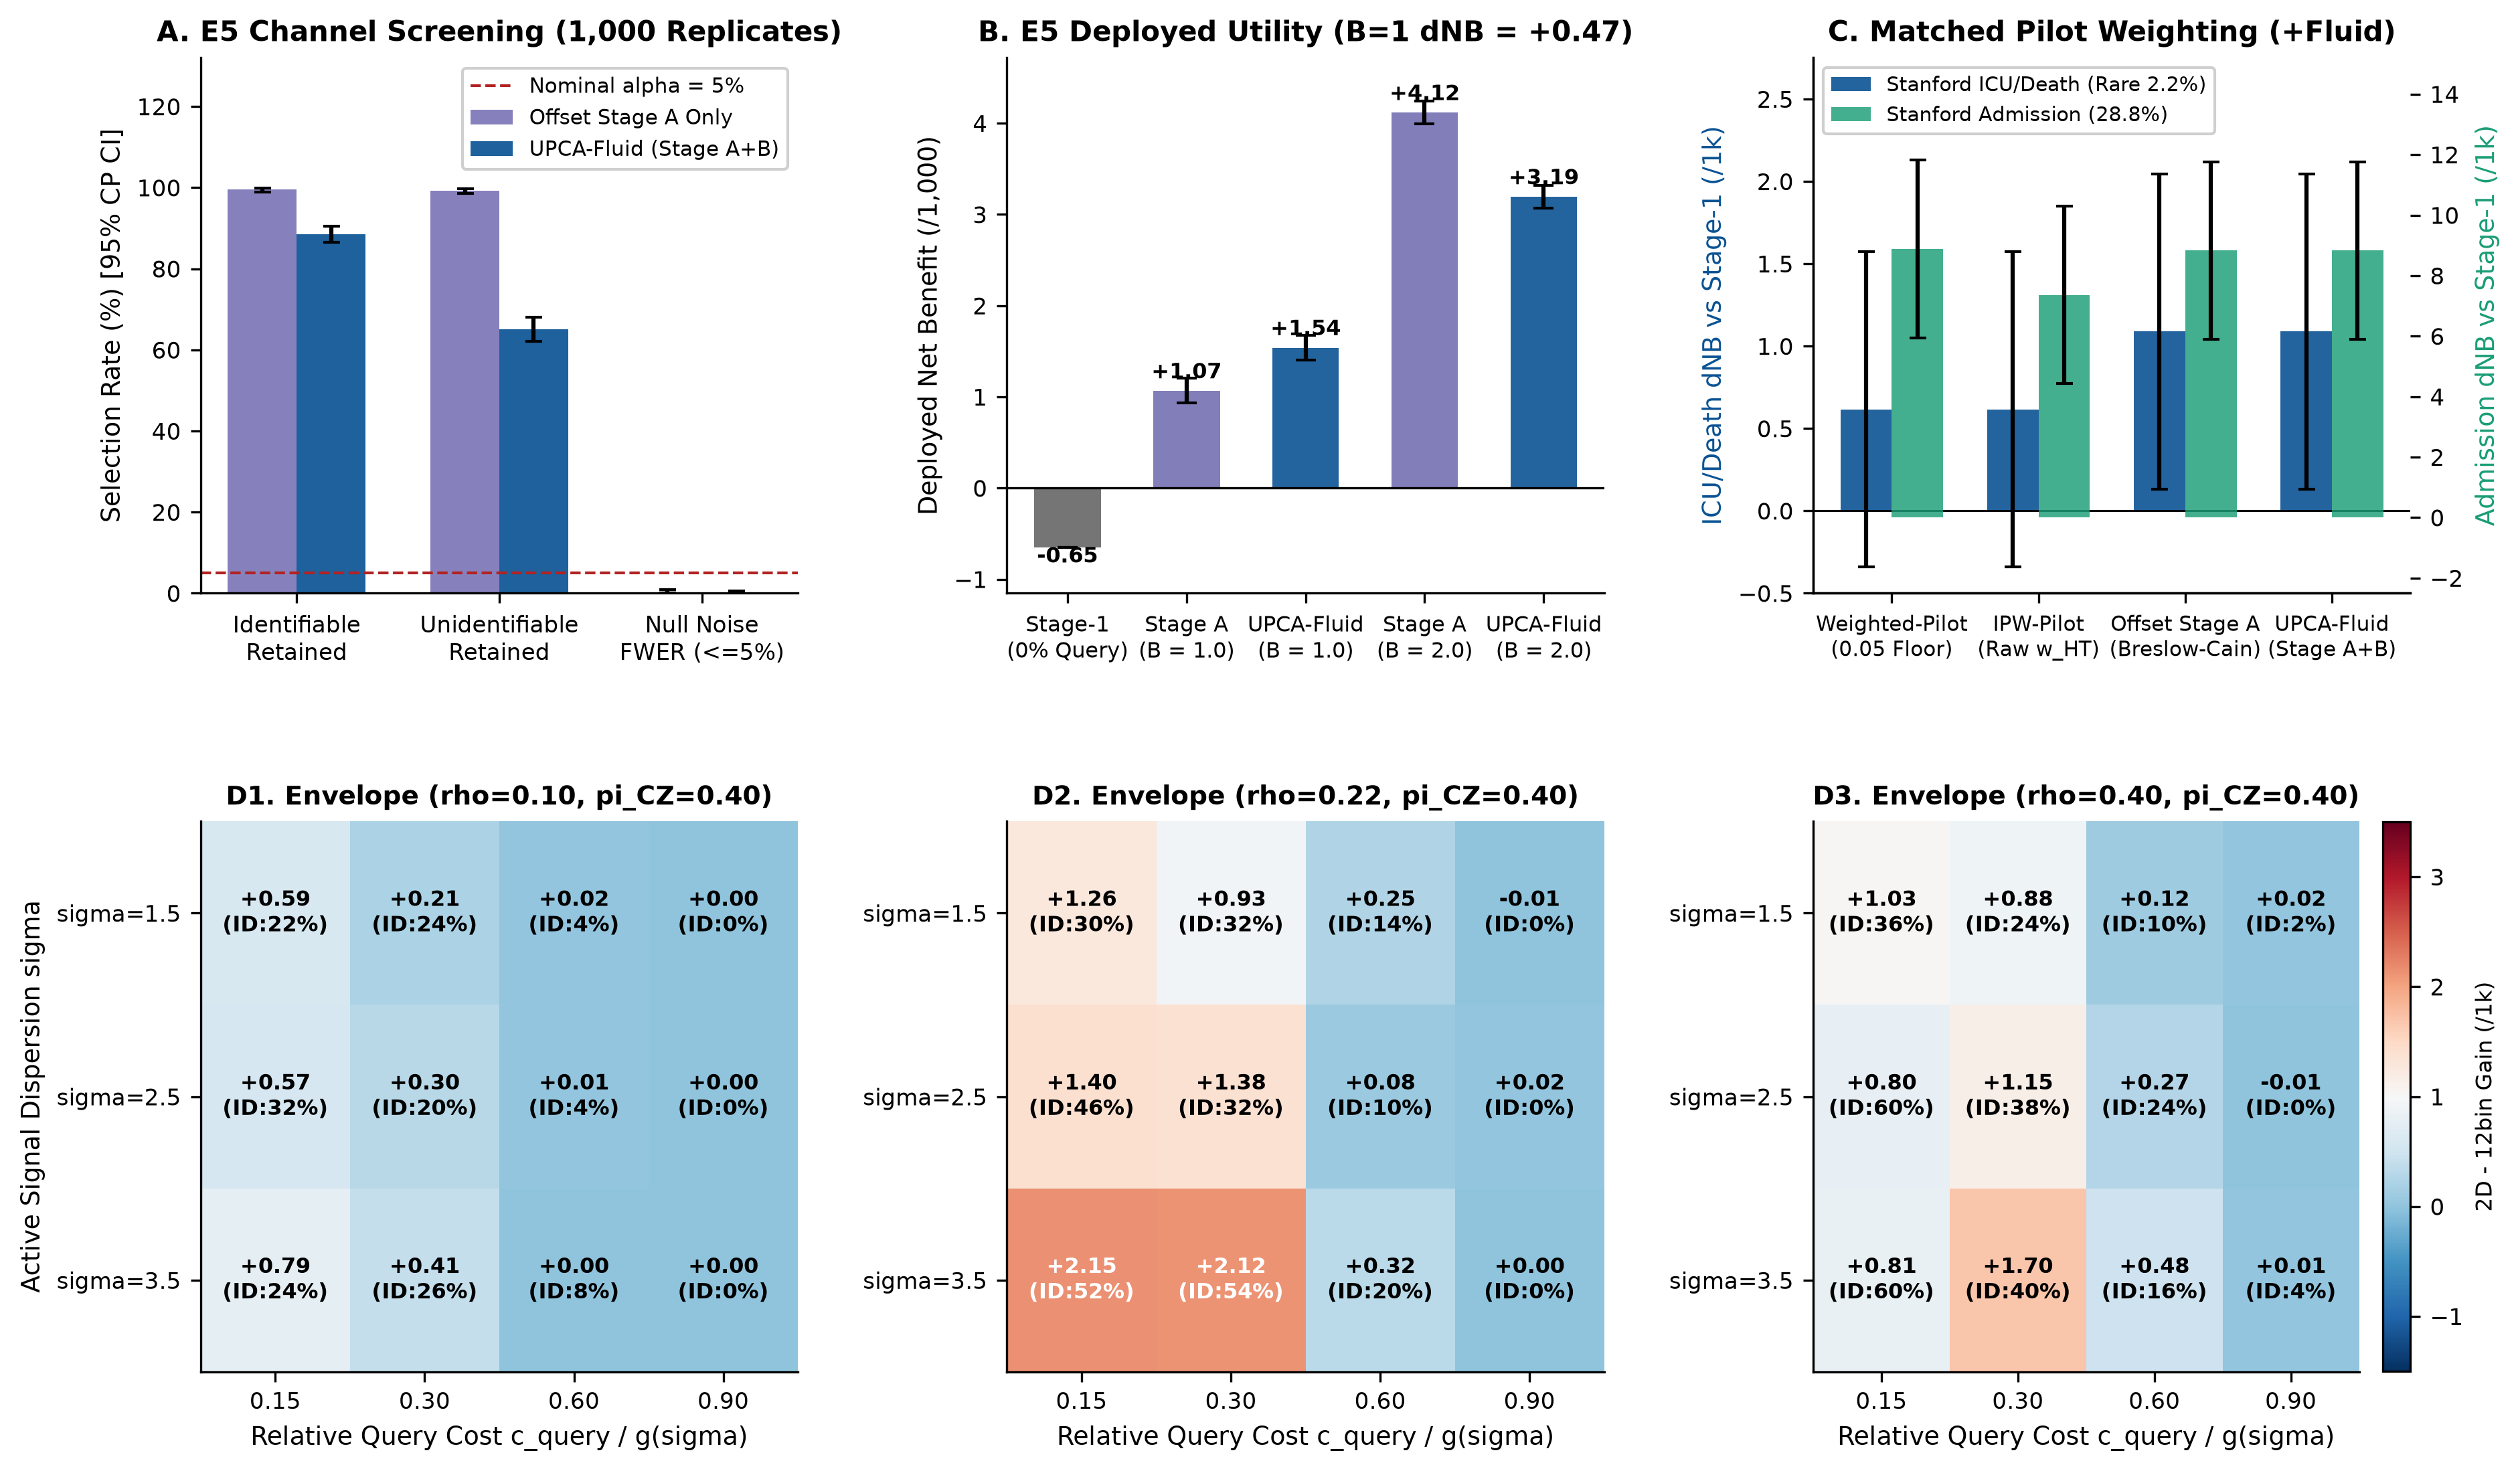
\includegraphics[width=\textwidth]{fig1_operating_envelope_and_regime.png}
\caption{Synthetic operating envelope, split-pilot FWER/power trade-off, and repeated-pilot discovery concordance. \textbf{(A)} $1{,}000$-replicate \texttt{E5} selection and null FWER alongside $200$-rep disjoint $50/50$ split-pilot confirmation. \textbf{(B)} Deployed Net Benefit under tight ($B=1.0$, $\Delta\operatorname{NB}=+0.47, p=1.4\times 10^{-11}$), flat-fee ($B=2.0$), and channel-scheduled ($B=2.0$) budgets. \textbf{(C)} Stanford ICU repeated-pilot top-$1$ oracle concordance across $\rho_{\text{pilot}} \in \{0.15, 0.20, 0.30\}$ ($500$ pilots at $\rho_{\text{pilot}}=0.20$: $87.4\%$ vs.\ $73.8\%$, $p=4.70\times 10^{-12}$; $200$-pilot $50/50$ split confirmation: $61.0\%$, FWER $1.0\%$). \textbf{(D1--D3)} $72$-cell ($3{,}600$-run) operating-envelope heatmaps at $\pi_{\text{CZ}}=0.40$.}
\label{fig:fig1}
\end{figure}

\subsection{Two-Phase Pilot Concordance, \texttt{Common-Panel Bagged VOI}, and Fee Sweeps}
\label{sec:clin_results}

Tables~\ref{tab:triad}--\ref{tab:channels} and Figures~\ref{fig:fig1}C, \ref{fig:fig2}, and \ref{fig:fig5}A--B report repeated-pilot discovery stability, $R=10$ \texttt{Common-Panel Bagged VOI} performance under \texttt{ChannelCostSchedule}, and query-cost sensitivity:

\begin{table}[t]
\centering
\caption{Primary held-out clinical evaluation using deployable $R=10$ \texttt{Common-Panel Bagged VOI} under \texttt{ChannelCostSchedule} ($B=10{,}000$ patient-cluster bootstraps; floor $0.0002$; canonical single-split and \texttt{Union-Panel}/\texttt{Sym.\ Ens.}/\texttt{Per-Split} estimands in Appendix Table~\ref{tab:estimands_supp}).}
\label{tab:triad}
\vspace{4pt}
\resizebox{\textwidth}{!}{%
\begin{tabular}{lcccccccc}
\toprule
\textbf{Task} & \textbf{Full 100\% All-$M$} & \textbf{S1 ($0\%$)} & \textbf{Bound.\ Unc.} & \textbf{\texttt{CMI+GBDT}} & \textbf{\texttt{UPCA-Fluid}} & \textbf{\texttt{UPCA} vs.\ Full-All} & \textbf{\texttt{UPCA} vs.\ S1} & \textbf{\texttt{Covert-CMI} AFA} \\
(Prev., $\tau^*$) & $\operatorname{NB}$ ($C$) & $\operatorname{NB}$ & $\operatorname{NB}$ ($q\%$) & $\operatorname{NB}$ ($q\%, C$) & $\operatorname{NB}$ ($q\%, C, R_{\text{CZ}}$) & $\Delta\operatorname{NB}$ [95\% CI] ($p_{\text{DH}}$) & $\Delta\operatorname{NB}$ [95\% CI] ($p_{\text{DH}}$) & Split / Maj.\ ($\Delta_{\text{Maj}}, p_{\text{DH}}$) \\
\midrule
1.\ Stanf.\ ICU & $+5.52$ ($.083$) & $+8.87$ & $+8.84$ ($19.1\%$) & $+9.09$ ($21.1\%, .038$) & $\mathbf{+9.00}$ ($19.1\%, .031, .004$) & $\mathbf{+3.48}$ [$+2.61,+4.32$] ($\mathbf{.0002}$) & $+0.12$ [$-0.67,+0.91$] ($.758$) & $+8.51$ / $+7.60$ ($\mathbf{+1.39, .0008}$) \\
2.\ Stanf.\ Admit & $+188.59$ ($.069$) & $+189.75$ & $+195.28$ ($54.0\%$) & $+194.05$ ($52.4\%, .034$) & $\mathbf{+195.09}$ ($54.0\%, .026, .036$) & $\mathbf{+6.51}$ [$+3.74,+9.19$] ($\mathbf{.0002}$) & $\mathbf{+5.35}$ [$+2.08,+8.65$] ($\mathbf{.0008}$) & $+191.25^*$ / $+183.67$ ($\mathbf{+11.43, .0002}$) \\
3.\ Stanf.\ Bounce & $+2.56$ ($.069$) & $+1.41$ & $+2.89$ ($72.7\%$) & $+3.35$ ($70.6\%, .014$) & $\mathbf{+2.91}$ ($72.7\%, .010, .122$) & $+0.36$ [$-1.05,+1.66$] ($.598$)$^\dagger$ & $+1.50$ [$-0.08,+3.20$] ($.064$)$^\ddagger$ & $+3.00$ / $+2.07$ ($+0.85, .237$) \\
4.\ BWH 30d Death & $+11.76$ ($.026$) & $+10.95$ & $+11.87$ ($33.8\%$) & $+12.18$ ($33.8\%, .016$) & $\mathbf{+12.02}$ ($33.8\%, .016, .000$) & $+0.26$ [$-0.47,+0.93$] ($.433$)$^\dagger$ & $+1.07$ [$-0.32,+2.53$] ($.137$) & $+11.08$ / $+11.53$ ($+0.50, .489$) \\
5.\ BWH 10d Rev.\ & $+4.33$ ($.026$) & $+3.13$ & $+5.10$ ($34.4\%$) & $+4.52$ ($34.6\%, .015$) & $\mathbf{+4.84}$ ($34.4\%, .010, .104$) & $+0.51$ [$-1.12,+2.13$] ($.538$)$^\dagger$ & $\mathbf{+1.71}$ [$+0.33,+3.19$] ($\mathbf{.0182}$) & $+4.16$ / $+3.03$ ($\mathbf{+1.81, .0126}$) \\
6.\ NTUH SCA & $-1.40$ ($.047$) & $+0.18$ & $+0.18$ ($0.0\%$) & $+0.18$ ($0.0\%, .000$) & $\mathbf{+0.18}$ ($0.0\%, .000, .000$) & $\mathbf{+1.58}$ [$+0.28,+2.74$] ($\mathbf{.0208}$) & $+0.00$ [exact tie] ($1.00$) & $-0.08^*$ / $-0.06$ ($\mathbf{+0.24, .0118}$) \\
\bottomrule
\multicolumn{9}{l}{\footnotesize $^*$Per-split \texttt{UPCA} vs.\ \texttt{Covert-CMI} also significant on Admission ($+3.84, p_{\text{DH}}=0.0008$) and NTUH ($+0.26, p_{\text{DH}}=0.0032$). $^\dagger$At $3.0\times$ fees, \texttt{UPCA} beats Full-All on Bounce ($+4.44, p=.0002$) \& D30 ($+1.68, p=.0002$).}\\
\multicolumn{9}{l}{\footnotesize $^\ddagger$Canonical single-split Bounceback \texttt{UPCA} vs.\ Stage-1 is $+2.63$ ($[+0.87, +4.51], p_{\text{DH}}=0.0026$). All $R=10$ \texttt{UPCA} vs.\ \texttt{CMI+GBDT} and vs.\ \texttt{Bound.\ Unc.} $95\%$ CIs cross $0$ ($p_{\text{DH}} \ge 0.129$).}
\end{tabular}%
}
\end{table}

\begin{table}[t]
\centering
\caption{Locked Stage-2 panels $\mathcal{S}_{\text{common}}$ under \texttt{ChannelCostSchedule} ($C$ in $C_{\text{FP}}$ units), $R=10$ split selection counts, disjoint $50/50$ split-pilot panels, and matched-GBDT \texttt{Covert-CMI} / \texttt{Direct-VOI} null-noise query rates (abbreviations: \texttt{mon}=2h monitor, \texttt{ren}=renal/elyte, \texttt{lac}=lactate/cardiac, \texttt{lft}=LFT/coag, \texttt{cbc}=CBC, \texttt{pmh}=CDW PMH, \texttt{med}=CDW meds, \texttt{isc}=ECG ischemia, \texttt{rhy}=ECG rhythm, \texttt{wf}=ECG waveform).}
\label{tab:channels}
\vspace{4pt}
\resizebox{\textwidth}{!}{%
\begin{tabular}{lllllll}
\toprule
\textbf{Primary Task ($B$)} & \textbf{\texttt{Global-CMI}} ($C$; $R=10$ Counts) & \textbf{\texttt{Weighted-CZ}} ($C$; $R=10$) & \textbf{Stage-A Offset} & \textbf{$50/50$ Split-Pilot} ($C$) & \textbf{\texttt{UPCA-Fluid}} ($C$; $R=10$; Null $0\%$) & \textbf{\texttt{Covert-CMI} / \texttt{Direct-VOI}} Null $q\%$ \\
\midrule
1.\ Stanf.\ ICU ($3.0$) & \texttt{mon,ren,lac} ($.0375$; $10,10,6$) & \texttt{ren,lac} ($.0308$; \texttt{mon} $9$, \texttt{ren} $9$) & \texttt{ren,mon,lac} & \texttt{lac} ($.0204$) & \texttt{ren,lac} ($.0308$; \texttt{ren} $7$, \texttt{mon} $6$) & $1.6\%$ / $1.1\%$ \\
2.\ Stanf.\ Admit ($3.0$) & \texttt{pmh,lac,cbc,mon} ($.0337$; $10,10,5$) & \texttt{pmh,lft,lac} ($.0297$; $10,9,4$) & \texttt{pmh,lft,cbc} & \texttt{pmh,cbc,lft} ($.0262$) & \texttt{pmh,lft,cbc} ($.0262$; $10,9,8$) & $0.05\%$ / $0.05\%$ \\
3.\ Stanf.\ Bounce ($3.0$) & \texttt{pmh,med} ($.0138$; $10,4$) & \texttt{pmh,lac} ($.0208$; $10,2$) & \texttt{pmh,lac} & \texttt{pmh} ($.0100$) & \texttt{pmh} ($.0100$; \texttt{pmh} $10$, \texttt{med} $6$) & $9.0\%$ / $14.2\%$ \\
4.\ BWH 30d Death ($1.8$) & \texttt{wf} ($.0156$; \texttt{wf} $10$) & \texttt{wf} ($.0156$; \texttt{wf} $10$) & \texttt{wf} & \texttt{wf} ($.0156$) & \texttt{wf} ($.0156$; \texttt{wf} $6/10$ kept) & $5.8\%$ / $1.3\%$ \\
5.\ BWH 10d Rev.\ ($1.8$) & \texttt{isc,rhy} ($.0150$; \texttt{isc} $10$, \texttt{wf} $5$) & \texttt{isc,wf} ($.0206$; \texttt{isc} $10$, \texttt{wf} $2$) & \texttt{isc,wf} & \texttt{isc} ($.0100$) & \texttt{isc} ($.0100$; \texttt{isc} $9$, \texttt{rhy} $3$) & $4.2\%$ / $3.3\%$ \\
6.\ NTUH SCA ($1.8$) & $\emptyset$ ($.0000$; \texttt{avr} $3/10$) & $\emptyset$ ($.0000$; \texttt{avr} $1/10$) & $\emptyset$ & $\emptyset$ ($.0000$) & $\emptyset$ ($.0000$; $9/10$ abstain) & $1.5\%$ / $0.3\%$ \\
\bottomrule
\end{tabular}%
}
\end{table}

\begin{enumerate}
  \item \textbf{Repeated-Pilot Discovery Concordance ($500$ Pilots) and Split-Pilot Confirmation ($200$ Pilots):} On Stanford $2\text{h}$ ICU/mortality ($\mathcal{D}_{\text{train}}=69{,}022$; full-cohort cost-normalized oracle top-$1$ channel \texttt{monitor\_numerics\_2h}), $500$ repeated $20\%$ Collision-Zone pilots show that unweighted Breslow--Cain offset GBDTs raise top-$1$ oracle concordance from $73.8\%$ ($369/500$, \texttt{Weighted-CZ}) and $67.6\%$ ($338/500$, \texttt{IPW}) to \textbf{$87.4\%$ ($437/500$, $[84.2\%, 90.2\%]$; paired $+13.6\%$, $[+9.8\%, +17.4\%]$, exact McNemar $p=4.70\times 10^{-12}$)}, recover \texttt{monitor\_numerics\_2h} in $98.0\%$ ($147/150$) vs.\ $88.0\%$ ($p=2.75\times 10^{-4}$) of full $3$-step bundles, cut parametric lactate slope variance by $34.5\%$ vs.\ IPW ($0.01519$ vs.\ $0.01876$; \citealp{tao2017efficient}), and hold across $\rho_{\text{pilot}} \in \{0.15, 0.20, 0.30\}$ ($74.0\%$ vs.\ $61.0\%$ at $0.15$; $100.0\%$ vs.\ $96.5\%$ at $0.30$; Appendix Table~\ref{tab:r15_supp}). Auditing $200$ additional pilots at $\rho_{\text{pilot}}=0.20$ with two Gaussian null channels appended confirms $0.0\%$ ($0/200$) cross-fitted null FWER vs.\ $1.0\%$ ($2/200$, $[0.12\%, 3.57\%]$) under disjoint $50/50$ split-pilot confirmation, while quantifying the split-pilot sample-halving power cost: top-$1$ concordance drops from $82.0\%$ to $61.0\%$ (McNemar $p=1.0\times 10^{-6}$) and bundle recovery from $91.5\%$ to $48.5\%$ ($p < 10^{-18}$; Figure~\ref{fig:fig1}C). Moreover, our earlier Stanford ICU \texttt{seed=44} within-stratum independence flag ($p=0.0270$ at truncated raw rank $19$) is confirmed to be a raw-unit scaling artifact: across $500$ random seeds, \texttt{sample\_pilot} rejects at $4.8\%$ (raw) and $5.0\%$ (standardized), and full-rank ($\text{df}=72$) correlation-standardized Mahalanobis testing yields $\chi^2=70.21, p=0.5376$ (design-permutation $p=0.517$).
  \item \textbf{Selective Querying vs.\ Full $100\%$ Stage-2, Neutral ICU Contrast vs.\ Stage-1, and Cost-Multiplier Sweeps:} Under \texttt{ChannelCostSchedule}, Stage-B OOF screening on canonical Stanford ICU prunes \texttt{monitor\_numerics\_2h} ($z_{\text{marg}}=1.115 < 1.282$), locking \texttt{[renal\_elyte, lactate\_cardiac]} ($C=0.0308$ vs.\ $0.0375$ unpruned and $0.0829$ for all $8$ channels). Consequently, deployable $R=10$ \texttt{Common-Panel Bagged VOI} ($+9.00/1{,}000, q=19.1\%$) substantially outperforms \textbf{\texttt{Full 100\% All-8} querying ($+5.52$, $\Delta=+3.48$ $[+2.61, +4.32], p_{\text{DH}}=0.0002$)} and \textbf{\texttt{Full 100\% Locked-Panel} querying ($+7.73$, $\Delta=+1.27$ $[+0.85, +1.60], p_{\text{DH}}=0.0004$)}, while its gain over zero-query $R=10$ Stage-1 ($+8.87$: $\Delta=+0.12$ $[-0.67, +0.91], p_{\text{DH}}=0.758$; canonical $+8.97$ vs.\ $+8.36, \Delta=+0.61, p_{\text{DH}}=0.200$; \texttt{Sym.\ Ens.} $+9.48$) lies below the $1.0/1{,}000$ reference $\texttt{MCID}$ and is statistically inconclusive (tying \texttt{Weighted-CZ} at $+9.00$, \texttt{CMI+GBDT} at $+9.09$ [$p_{\text{DH}}=0.768$], and matched-rate \texttt{Boundary Uncertainty} at $+8.84$ [$p_{\text{DH}}=0.287$]). Across the remaining five tasks, \texttt{Common-Panel Bagged VOI} beats both \texttt{Full 100\% All-8} ($\mathbf{+6.51}, p_{\text{DH}}=0.0002$) and Stage-1 ($\mathbf{+5.35}, p_{\text{DH}}=0.0008$) on \textbf{Stanford Admission}, beats Stage-1 above reference $\texttt{MCID}$ on \textbf{BWH $10\text{d}$ Stent/CABG} ($\mathbf{+1.71}$ $[+0.33, +3.19], p_{\text{DH}}=0.0182$), shows $+1.50$ ($p_{\text{DH}}=0.064$; canonical $+2.63, p_{\text{DH}}=0.0026$) on $72\text{h}$ Bounceback and $+1.07$ ($p_{\text{DH}}=0.137$) on BWH $30\text{d}$ Mortality, and cleanly abstains ($q=0.0\%, +0.18$) on \textbf{NTUH Pre-Arrest}, sparing $\mathbf{+1.58/1{,}000}$ ($p_{\text{DH}}=0.0208$) vs.\ \texttt{Full 100\% All-6} ($-1.40$). Sweeping assigned costs across $0.5\times\text{--}3.0\times$ (Figure~\ref{fig:fig5}A--B) monotonically reduces \texttt{UPCA} query rates ($24.4\%\to 10.1\%$ on ICU; $60.2\%\to 35.8\%$ on Admission) while widening gains over \texttt{Full 100\% All-$M$} from $+1.37$ ($0.5\times$) to $+11.98/1{,}000$ ($3.0\times$) on ICU and $+2.12$ to $+27.10/1{,}000$ on Admission, underscoring that Net Benefit advantages over universal testing depend directly on assigned channel fees.
  \item \textbf{Matched-GBDT \texttt{Covert-CMI} / \texttt{Direct-VOI} Scope and Scale-Invariant $R_{\text{CZ}}$:} Within matched random-mask LightGBM predictors, instancewise \texttt{Covert-CMI} and \texttt{Direct-VOI} query Gaussian null channels on $0.05\%\text{--}14.2\%$ of encounters per split (Table~\ref{tab:channels}), over-query Stanford Admission ($86.2\%$, losing by $+3.84$ per-split [$p_{\text{DH}}=0.0008$] and $+11.43$ under majority-mask [$p_{\text{DH}}=0.0002$]), and degrade under majority-mask consensus on Stanford ICU ($+7.60$ vs.\ $+9.00, \Delta=+1.39, p_{\text{DH}}=0.0008$) and BWH Revascularization ($+3.03$ vs.\ $+4.84, \Delta=+1.81, p_{\text{DH}}=0.0126$). Scale-invariant diagnostics explain why \texttt{UPCA-Fluid} and \texttt{CMI+GBDT} tie across all six tasks ($p_{\text{DH}} \ge 0.280$): Stage-2 physiology is largely homogeneous on Stanford ICU ($R_{\text{CZ}}=0.0038$, flip $0.02\%$), BWH Mortality ($R_{\text{CZ}}=0.0000$), and NTUH ($0.0000$), and contributes modestly ($R_{\text{CZ}} \in [0.0355, 0.1224]$, flips $0.85\%\text{--}1.95\%$) on Admission, Bounceback, and Revascularization, so the KL-gated specialist appropriately self-damps.
\end{enumerate}

\begin{figure}[t]
\centering
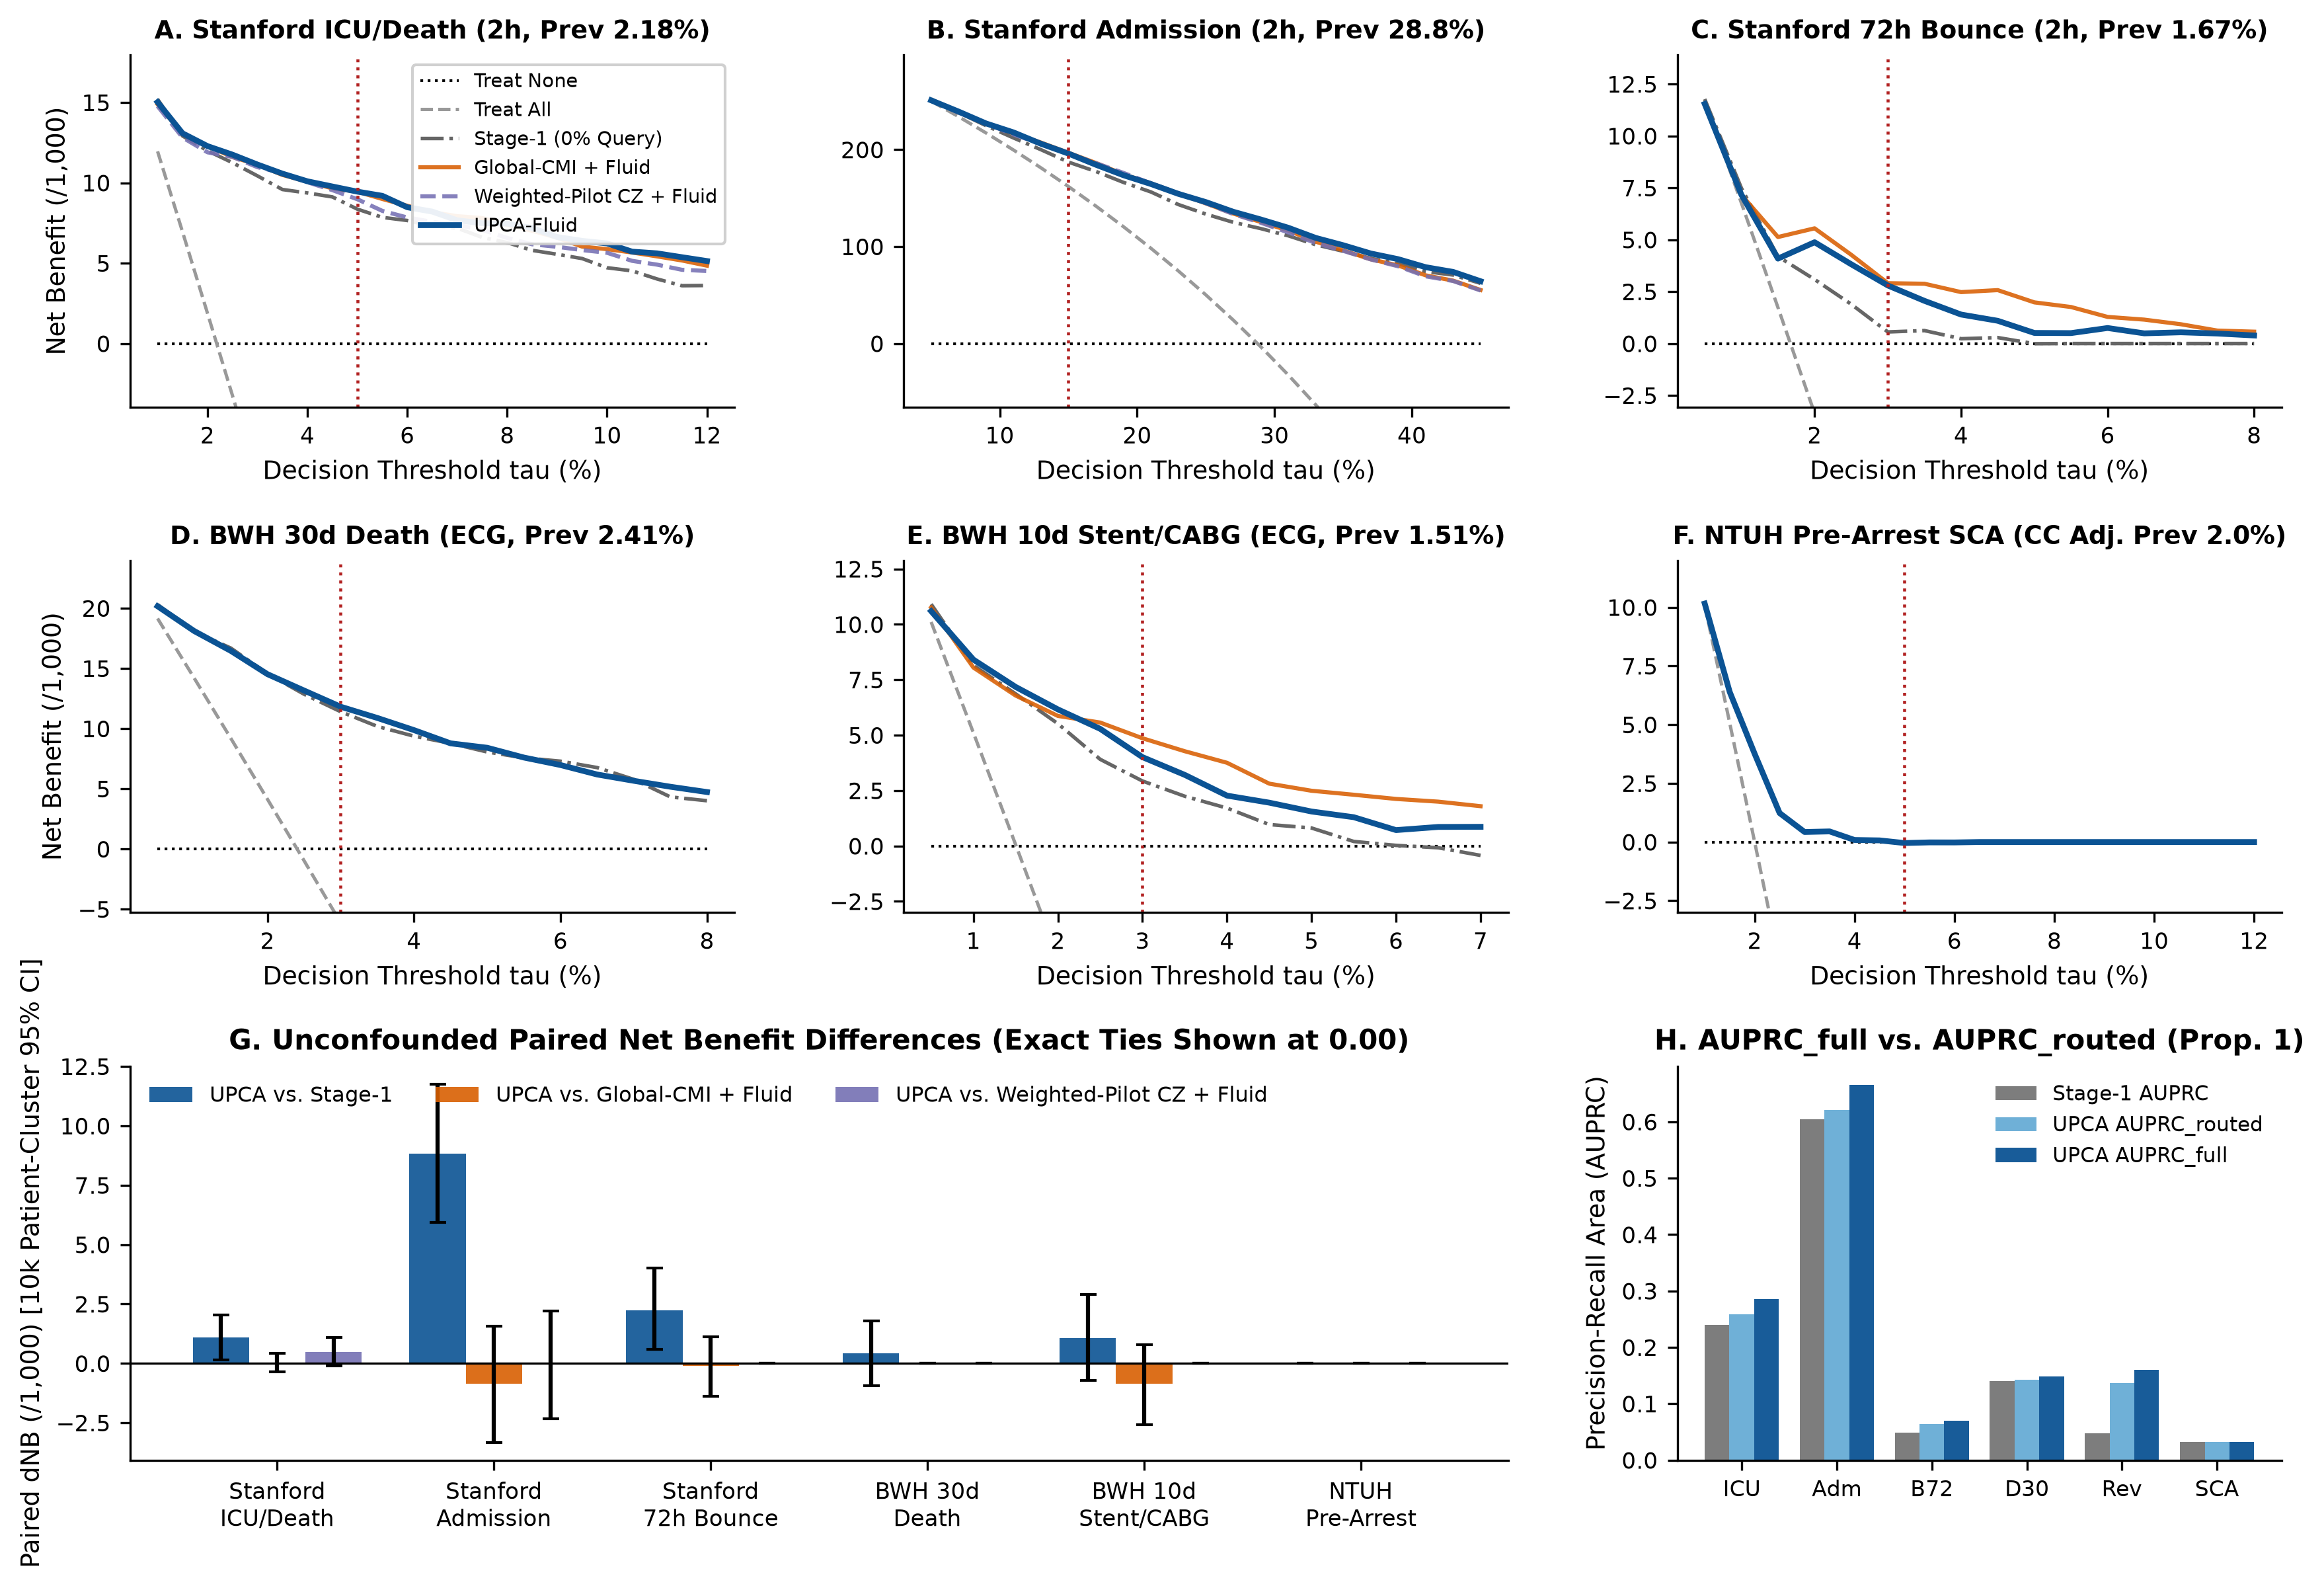
\includegraphics[width=\textwidth]{fig2_clinical_net_benefit_and_dca.png}
\caption{Vickers Decision Curves, $R=10$ \texttt{Common-Panel Bagged VOI} contrasts under \texttt{ChannelCostSchedule}, and precision--recall behavior across all six tasks. \textbf{(A--F)} Net Benefit curves $\operatorname{NB}(\tau)$ around $\tau^*$ (vertical dotted line). \textbf{(G)} $10{,}000$-replicate patient-cluster bootstrap $\Delta\operatorname{NB}$ ($95\%$ CIs) vs.\ \texttt{Full 100\% All-$M$}, Stage-1, matched-rate \texttt{Boundary Uncertainty}, and channel-billed \texttt{Covert-CMI}. \textbf{(H)} Stage-1, $\operatorname{AUPRC}_{\text{routed}}$, and $\operatorname{AUPRC}_{\text{full}}$ illustrating Proposition~\ref{prop:auprc_inversion}.}
\label{fig:fig2}
\end{figure}

\subsection{Missed-Case / Directional VOI Ledger, 4-Way Prior-Shift Taxonomy, and Subgroup Heterogeneity}
\label{sec:cal_safety_fairness}

\textbf{Missed-Case Trade-Offs, Pre-Fee vs.\ Fee-Saving Decomposition, and \texttt{Escalation-Only VOI} (Table~\ref{tab:icu_exchange}, Figure~\ref{fig:fig5}C):} Across all $N_{\text{test}}=10{,}486$ Stanford ICU arrivals ($229$ true events $= 21.84/1{,}000$), Table~\ref{tab:icu_exchange} exposes the exact clinical exchange rate behind selective Net Benefit. Relative to \texttt{Full 100\% All-8} querying at $\tau \in \{3\%, 5\%, 8\%, 10\%\}$ ($175, 154, 135, 127$ TPs), default two-sided \texttt{UPCA-Fluid} ($q=19.1\%$) catches $+3, +1, +11, +21$ more critical cases than zero-query Stage-1, yet misses \textbf{$16, 6, 5,$ and $5$ cases ($-9.1\%, -3.9\%, -3.7\%, -3.9\%$ sensitivity loss vs.\ \texttt{Full 100\% All-8})}. Algebraically, two-sided \texttt{UPCA-Fluid} incurs a small pre-fee decision loss against \texttt{Full 100\% All-8} ($\Delta\operatorname{NB}_{\text{pre-fee}} = -1.40, -0.58, -0.75, -1.10/1{,}000$) that is outweighed by large query-fee savings ($+2.38, +4.05, +6.70, +8.56/1{,}000$), producing positive net ledger gains of $\mathbf{+0.99, +3.48, +5.95,}$ and $\mathbf{+7.45/1{,}000}$ ($p_{\text{DH}} \le 0.038$). Crucially, switching to \textbf{\texttt{Escalation-Only VOI}} ($q=6.3\%\text{--}17.9\%$) misses \textbf{$0$ baseline Stage-1 cases} at every threshold, catches $+7, +9, +20,$ and $+26$ additional critical cases over Stage-1, and at $\tau^*=5.0\%$ ($156$ vs.\ $154$ TPs, $68.1\%$ vs.\ $67.3\%$ sensitivity, $\operatorname{NB}=+8.51$) and $\tau=8.0\%$ ($139$ vs.\ $135$ TPs) achieves \emph{higher sensitivity than universal 8-channel querying} by preventing Stage-2 de-escalation of high-risk triage presentations.

\begin{table}[t]
\centering
\caption{Stanford $2\text{h}$ ICU/mortality ($N_{\text{test}}=10{,}486$; $229$ true events $= 21.84/1{,}000$) missed-case, pre-fee vs.\ fee-saving, and directional VOI exchange ledger across $\tau \in \{3\%, 5\%, 8\%, 10\%\}$ ($R=10$ \texttt{Common-Panel Bagged VOI}, $B=10{,}000$ patient-cluster bootstraps).}
\label{tab:icu_exchange}
\vspace{4pt}
\resizebox{\textwidth}{!}{%
\begin{tabular}{llrrrrcccc}
\toprule
\textbf{$\tau$ (FP:TP)} & \textbf{Routing Policy} & \textbf{TP} (\textbf{Sens.}) & \textbf{Miss vs.\ All-8 / S1} & \textbf{FP} (\textbf{PPV}) & \textbf{Query $q\%$} & \textbf{Pre-Fee $\operatorname{NB}$} & \textbf{Fee Drag} & \textbf{$\Delta_{\text{pre}} + \Delta_{\text{fee}}$ vs.\ All-8} & \textbf{Net $\operatorname{NB}$ ($\Delta$ vs.\ All-8, $p_{\text{DH}}$)} \\
\midrule
\multirow{4}{*}{$3.0\%$ ($32.3\text{:}1$)}
  & Full 100\% All-8 & 175 (76.4\%) & 0 / $-19$ & 1,407 (11.1\%) & 100.0\% & $+12.54$ & $-2.56$ & $0.00 + 0.00$ & $+9.98$ (Ref.) \\
  & Stage-1 ($0\%$ Query) & 156 (68.1\%) & 19 / 0 & 1,609 (8.8\%) & 0.0\% & $+10.13$ & $0.00$ & $-2.41 + 2.56$ & $+10.13$ ($+0.16, .764$) \\
  & \texttt{UPCA} Two-Sided & 159 (69.4\%) & 16 ($-9.1\%$) / $-3$ & 1,363 (10.5\%) & 19.1\% & $+11.14$ & $-0.18$ & $-1.40 + 2.38$ & $\mathbf{+10.96}$ ($\mathbf{+0.99, .0380}^*$) \\
  & \texttt{UPCA} Escalation-Only & 163 (71.2\%) & 12 ($-6.9\%$) / $\mathbf{-7}$ & 1,772 (8.4\%) & 6.3\% & $+10.32$ & $-0.06$ & $-2.22 + 2.50$ & $+10.26$ ($+0.28, .528$) \\
\midrule
\multirow{5}{*}{$\mathbf{5.0\%}$ ($\mathbf{19.0\text{:}1}$)}
  & Full 100\% All-8 & 154 (67.3\%) & 0 / $-7$ & 957 (13.9\%) & 100.0\% & $+9.88$ & $-4.36$ & $0.00 + 0.00$ & $+5.52$ (Ref.) \\
  & Full 100\% Locked & 152 (66.4\%) & 2 ($-1.3\%$) / $-5$ & 1,025 (12.9\%) & 100.0\% & $+9.35$ & $-1.62$ & $-0.53 + 2.74$ & $+7.73$ ($\mathbf{+2.21, .0002}$) \\
  & Stage-1 ($0\%$ Query) & 147 (64.2\%) & 7 ($-4.5\%$) / 0 & 1,025 (12.5\%) & 0.0\% & $+8.87$ & $0.00$ & $-1.01 + 4.36$ & $+8.87$ ($\mathbf{+3.35, .0002}$) \\
  & \textbf{\texttt{UPCA} Two-Sided} & \textbf{148 (64.6\%)} & \textbf{6 ($\mathbf{-3.9\%}$) / $-1$} & \textbf{958 (13.4\%)} & \textbf{19.1\%} & $\mathbf{+9.31}$ & $\mathbf{-0.31}$ & $\mathbf{-0.58 + 4.05}$ & $\mathbf{+9.00}$ ($\mathbf{+3.48, .0002}$) \\
  & \textbf{\texttt{UPCA} Escalation-Only} & \textbf{156 (68.1\%)} & $\mathbf{-2}$ ($\mathbf{+1.3\%}$) / $\mathbf{-9}$ & 1,229 (11.3\%) & 12.0\% & $+8.71$ & $-0.19$ & $-1.17 + 4.17$ & $+8.51$ ($\mathbf{+2.99, .0002}$) \\
\midrule
\multirow{3}{*}{$8.0\%$ ($11.5\text{:}1$)}
  & Full 100\% All-8 & 135 (59.0\%) & 0 / $-16$ & 622 (17.8\%) & 100.0\% & $+7.72$ & $-7.21$ & $0.00 + 0.00$ & $+0.51$ (Ref.) \\
  & \texttt{UPCA} Two-Sided & 130 (56.8\%) & 5 ($-3.7\%$) / $-11$ & 655 (16.6\%) & 19.1\% & $+6.97$ & $-0.51$ & $-0.75 + 6.70$ & $\mathbf{+6.46}$ ($\mathbf{+5.95, .0002}$) \\
  & \texttt{UPCA} Escalation-Only & \textbf{139 (60.7\%)} & $\mathbf{-4}$ ($\mathbf{+3.0\%}$) / $\mathbf{-20}$ & 780 (15.1\%) & 16.3\% & $+6.79$ & $-0.44$ & $-0.93 + 6.77$ & $+6.35$ ($\mathbf{+5.84, .0002}$) \\
\midrule
\multirow{3}{*}{$10.0\%$ ($9.0\text{:}1$)}
  & Full 100\% All-8 & 127 (55.5\%) & 0 / $-26$ & 473 (21.2\%) & 100.0\% & $+7.10$ & $-9.21$ & $0.00 + 0.00$ & $-2.11$ (Ref.) \\
  & \texttt{UPCA} Two-Sided & 122 (53.3\%) & 5 ($-3.9\%$) / $-21$ & 532 (18.7\%) & 19.1\% & $+6.00$ & $-0.65$ & $-1.10 + 8.56$ & $\mathbf{+5.35}$ ($\mathbf{+7.45, .0002}$) \\
  & \texttt{UPCA} Escalation-Only & \textbf{127 (55.5\%)} & \textbf{0 ($0.0\%$)} / $\mathbf{-26}$ & 599 (17.5\%) & 17.9\% & $+5.76$ & $-0.61$ & $-1.34 + 8.60$ & $+5.15$ ($\mathbf{+7.26, .0002}$) \\
\bottomrule
\multicolumn{10}{l}{\footnotesize $^*$At $\tau=3.0\%$, \texttt{UPCA} Two-Sided also significantly exceeds Stage-1 ($+0.83$ [$+0.20, +1.46$], $p_{\text{DH}}=0.0102$). Negative ``Miss'' values indicate additional true cases caught over reference.}
\end{tabular}%
}
\end{table}

\begin{figure}[t]
\centering
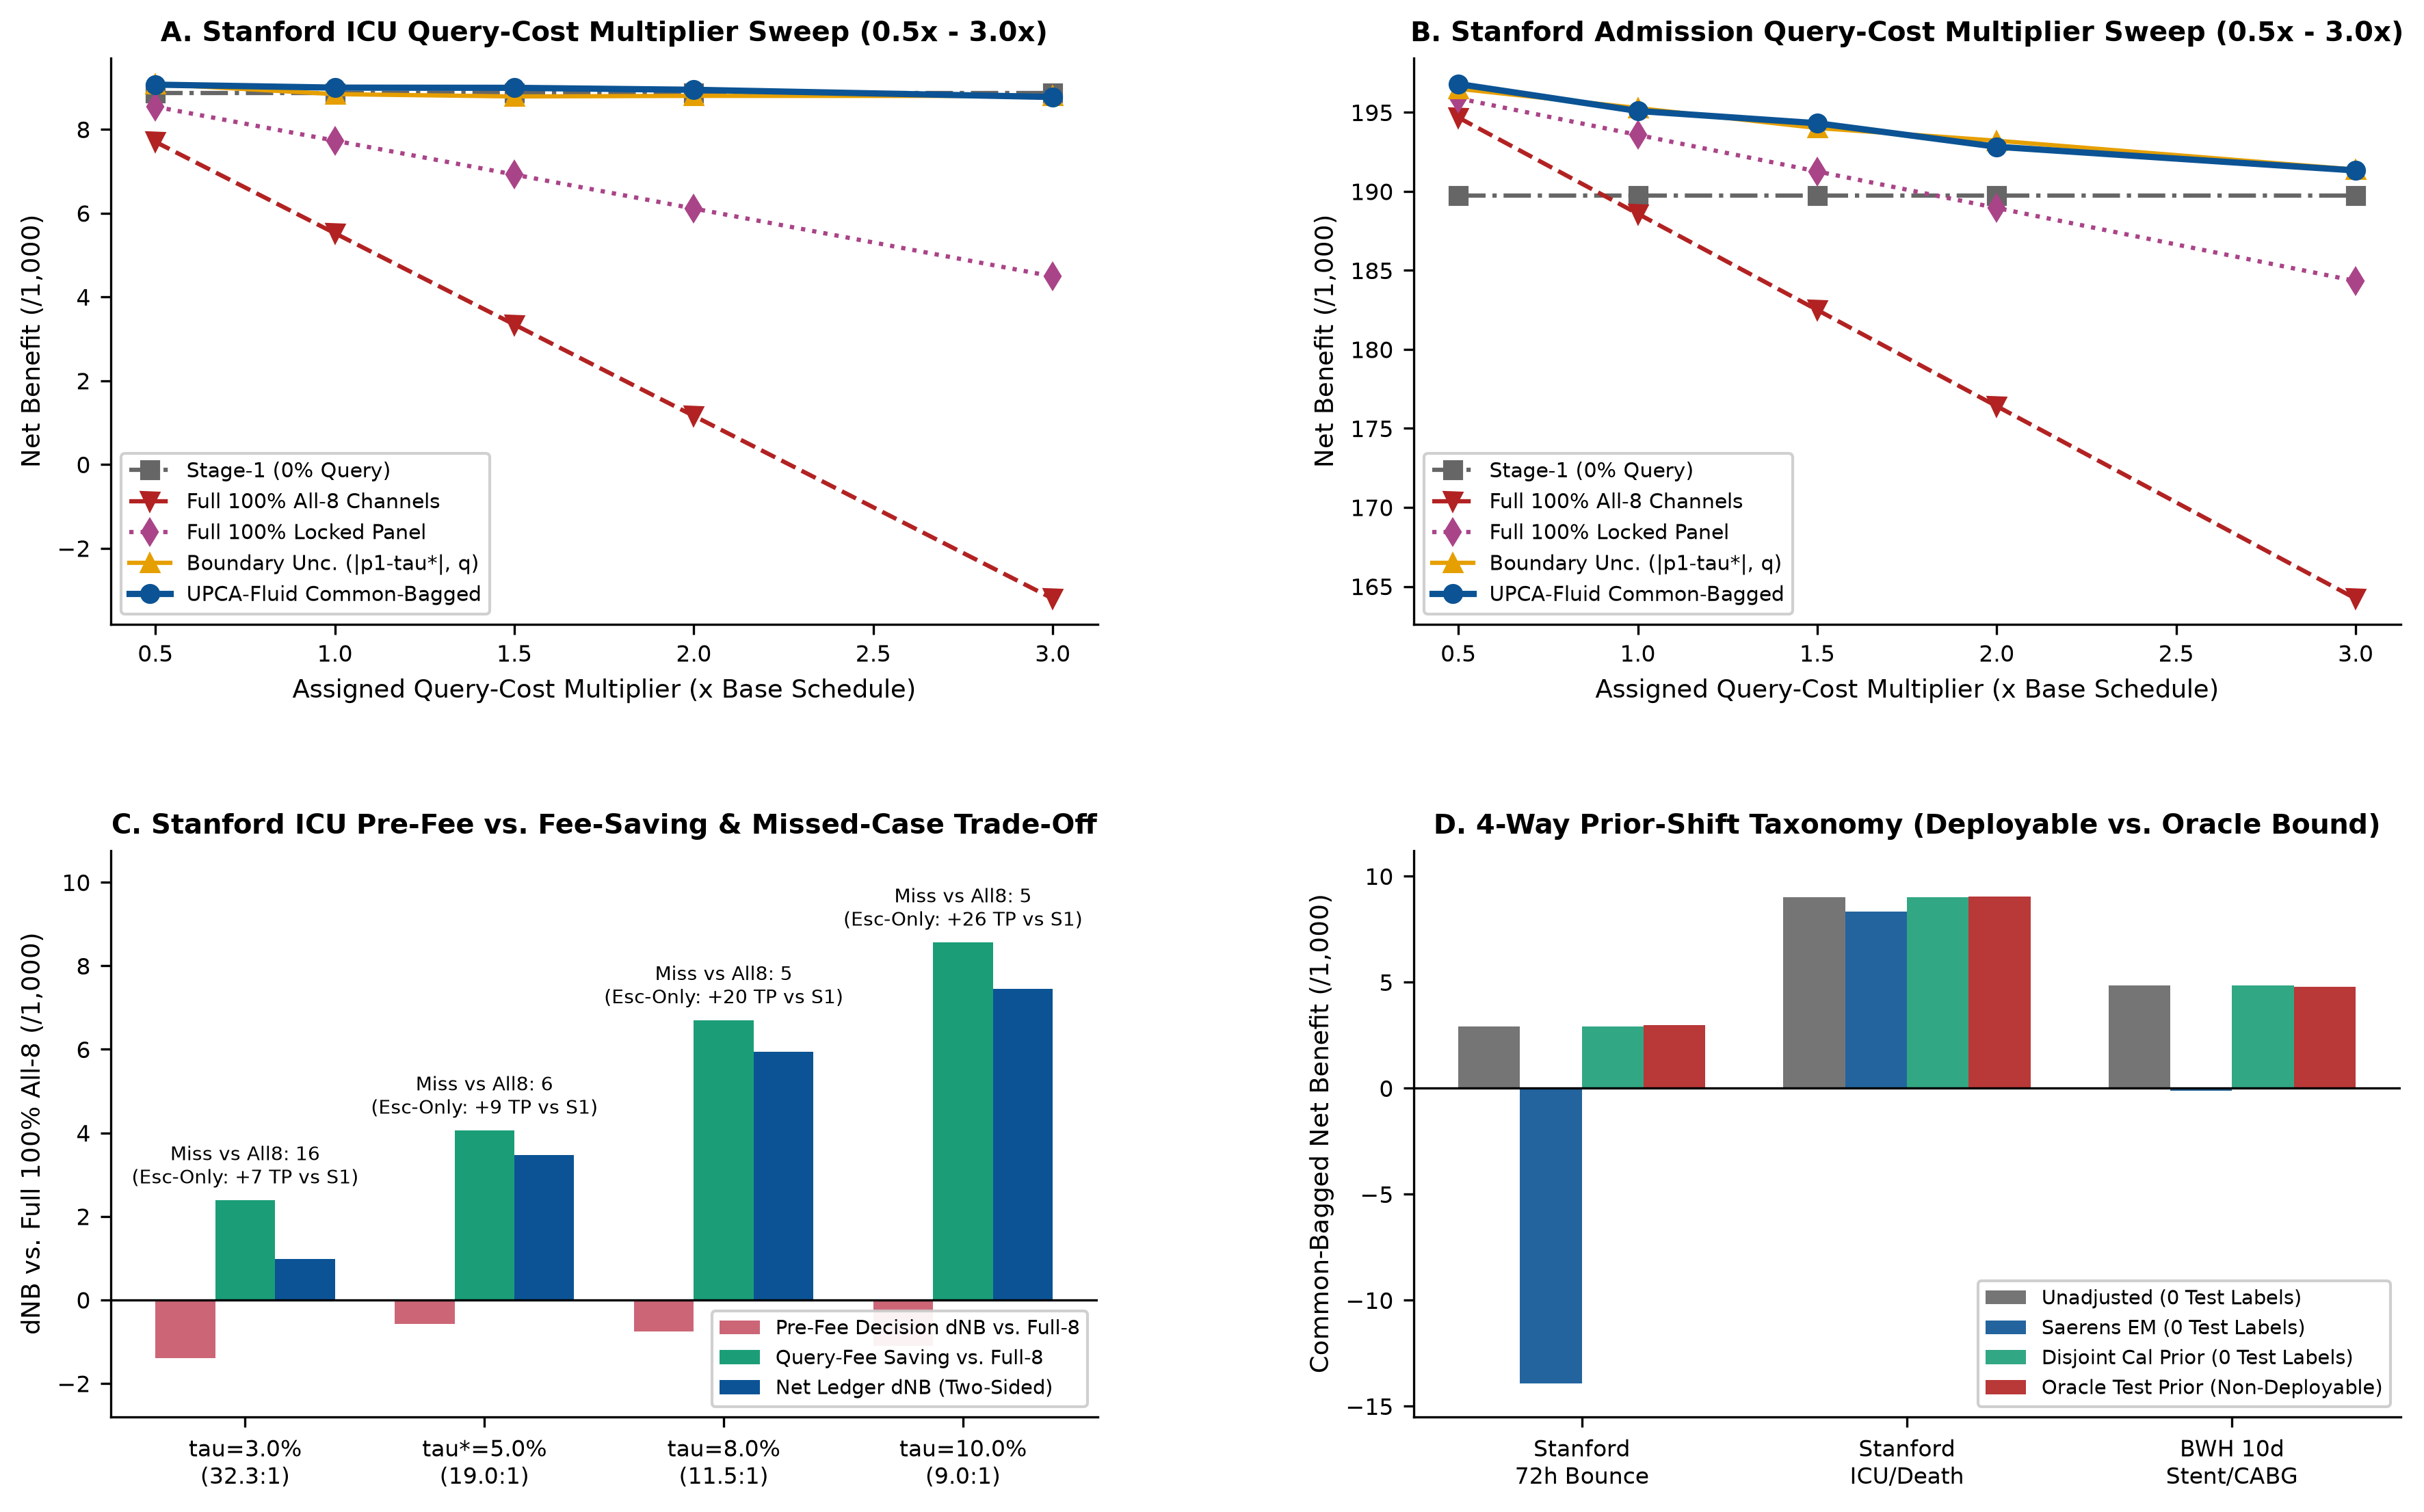
\includegraphics[width=\textwidth]{fig5_fee_sweep_and_missed_case_ledger.png}
\caption{Query-cost sensitivity, pre-fee vs.\ fee-saving decomposition, and 4-way prior-shift taxonomy. \textbf{(A--B)} $5$-point cost-multiplier sweep ($0.5\times\text{--}3.0\times$) on Stanford ICU/mortality and Inpatient Admission. \textbf{(C)} Stanford ICU decomposition of $\Delta\operatorname{NB}$ vs.\ \texttt{Full 100\% All-8} into pre-fee decision loss and query-fee savings alongside missed cases and \texttt{Escalation-Only VOI} extra true positives vs.\ Stage-1. \textbf{(D)} 4-way prior-shift taxonomy contrasting zero-test-label deployable estimators against the non-deployable Oracle $\pi_{\text{test}}$ bound.}
\label{fig:fig5}
\end{figure}

\textbf{Calibration and 4-Way Prior-Shift Taxonomy (Figure~\ref{fig:fig3}, Figure~\ref{fig:fig5}D, Table~\ref{tab:prior_shift}):} Unadjusted routed probabilities maintain near-zero calibration-in-the-large ($\operatorname{CITL} \in [-0.102, +0.108]$) and low spline $\operatorname{ICI} \in [0.0018, 0.0054]$ \citep{vancalster2019calibration,austin2019integrated}. Retiring our earlier draft's ``label-free'' $\pi_{\text{eval}}$ alignment (which inadvertently plugged realized $\pi_{\text{test}}$ into $72\text{h}$ Bounceback), Table~\ref{tab:prior_shift} compares three strictly zero-test-label deployable rules against the non-deployable Oracle $\pi_{\text{test}}$ upper bound. Under rare-event overlap ($1.5\%\text{--}2.2\%$ prevalence) and mild calibration slope deviation ($1.12\text{--}1.76$), unlabeled \citet{saerens2002adjusting} EM ($0$ test labels) is weakly identified and diverges toward boundary fixed points ($\hat{\pi}_{\text{EM}}=21.0\%$ on Bounceback $\to \operatorname{NB}=-13.93$; $\hat{\pi}_{\text{EM}}=10^{-5}$ on BWH Revascularization $\to \operatorname{NB}=-0.11$), whereas both \textbf{Unadjusted} and \textbf{Disjoint $\mathcal{D}_{\text{cal}}$ Prior Alignment} ($0$ test labels) preserve $\operatorname{ICI} \le 0.0045$ and statistically tie the non-deployable Oracle $\pi_{\text{test}}$ bound across all four rare cohorts ($|\Delta\operatorname{NB}| \le 0.07/1{,}000, p_{\text{DH}} \ge 0.743$).

\begin{table}[t]
\centering
\caption{Four-way prior-shift and intercept-recalibration taxonomy ($R=10$ \texttt{Common-Panel Bagged VOI}), strictly separating zero-test-label deployable estimators from the non-deployable Oracle $\pi_{\text{test}}$ upper bound ($B=10{,}000$ patient-cluster bootstraps).}
\label{tab:prior_shift}
\vspace{4pt}
\resizebox{\textwidth}{!}{%
\begin{tabular}{lccccccc}
\toprule
\textbf{Rare-Event Clinical Task} & \textbf{$\pi_{\text{cal}}$ / $\pi_{\text{test}}$} & \textbf{Unadjusted ($0$ Test Lbls)} & \textbf{Unlabeled Saerens EM ($0$ Lbls)} & \textbf{Disjoint $\mathcal{D}_{\text{cal}}$ Prior ($0$ Lbls)} & \textbf{Oracle $\pi_{\text{test}}$ Bound (Leaks Lbls)} & \textbf{Oracle $-$ Unadj.} \\
 &  & $\operatorname{NB}$ (\texttt{CITL}, \texttt{ICI}) & $\hat{\pi}_{\text{EM}}$ : $\operatorname{NB}$ (\texttt{CITL}, \texttt{ICI}) & $\operatorname{NB}$ (\texttt{CITL}, \texttt{ICI}) & $\operatorname{NB}$ (\texttt{CITL}, \texttt{ICI}) & $\Delta\operatorname{NB}$ ($p_{\text{DH}}$) \\
\midrule
3.\ Stanford 72h Bounceback & $1.54\% / 1.67\%$ & $+2.91$ ($+.017, .0040$) & $20.96\%$ : $-13.93$ ($-2.75, .1828$) & $+2.90$ ($+.015, .0040$) & $+2.99$ ($+.000, .0041$) & $+0.07$ ($0.745$) \\
1.\ Stanford ICU/Mortality & $2.24\% / 2.18\%$ & $+9.00$ ($-.102, .0035$) & $3.33\%$ : $+8.33$ ($-.446, .0099$) & $+9.00$ ($-.102, .0035$) & $+9.03$ ($-.014, .0027$) & $+0.03$ ($0.809$) \\
5.\ BWH 10d Stent/CABG & $1.47\% / 1.51\%$ & $+4.84$ ($+.108, .0018$) & $0.001\%$ : $-0.11$ ($+7.32, .0151$) & $+4.84$ ($+.108, .0018$) & $+4.78$ ($+.004, .0014$) & $-0.06$ ($0.743$) \\
6.\ NTUH Pre-Arrest SCA & $2.00\% / 2.00\%$ & $+0.18$ ($+.014, .0045$) & $0.006\%$ : $+0.00$ ($+5.88, .0199$) & $+0.18$ ($+.015, .0045$) & $+0.18$ ($+.000, .0045$) & $+0.00$ ($1.000$) \\
\bottomrule
\end{tabular}%
}
\end{table}

\begin{figure}[t]
\centering
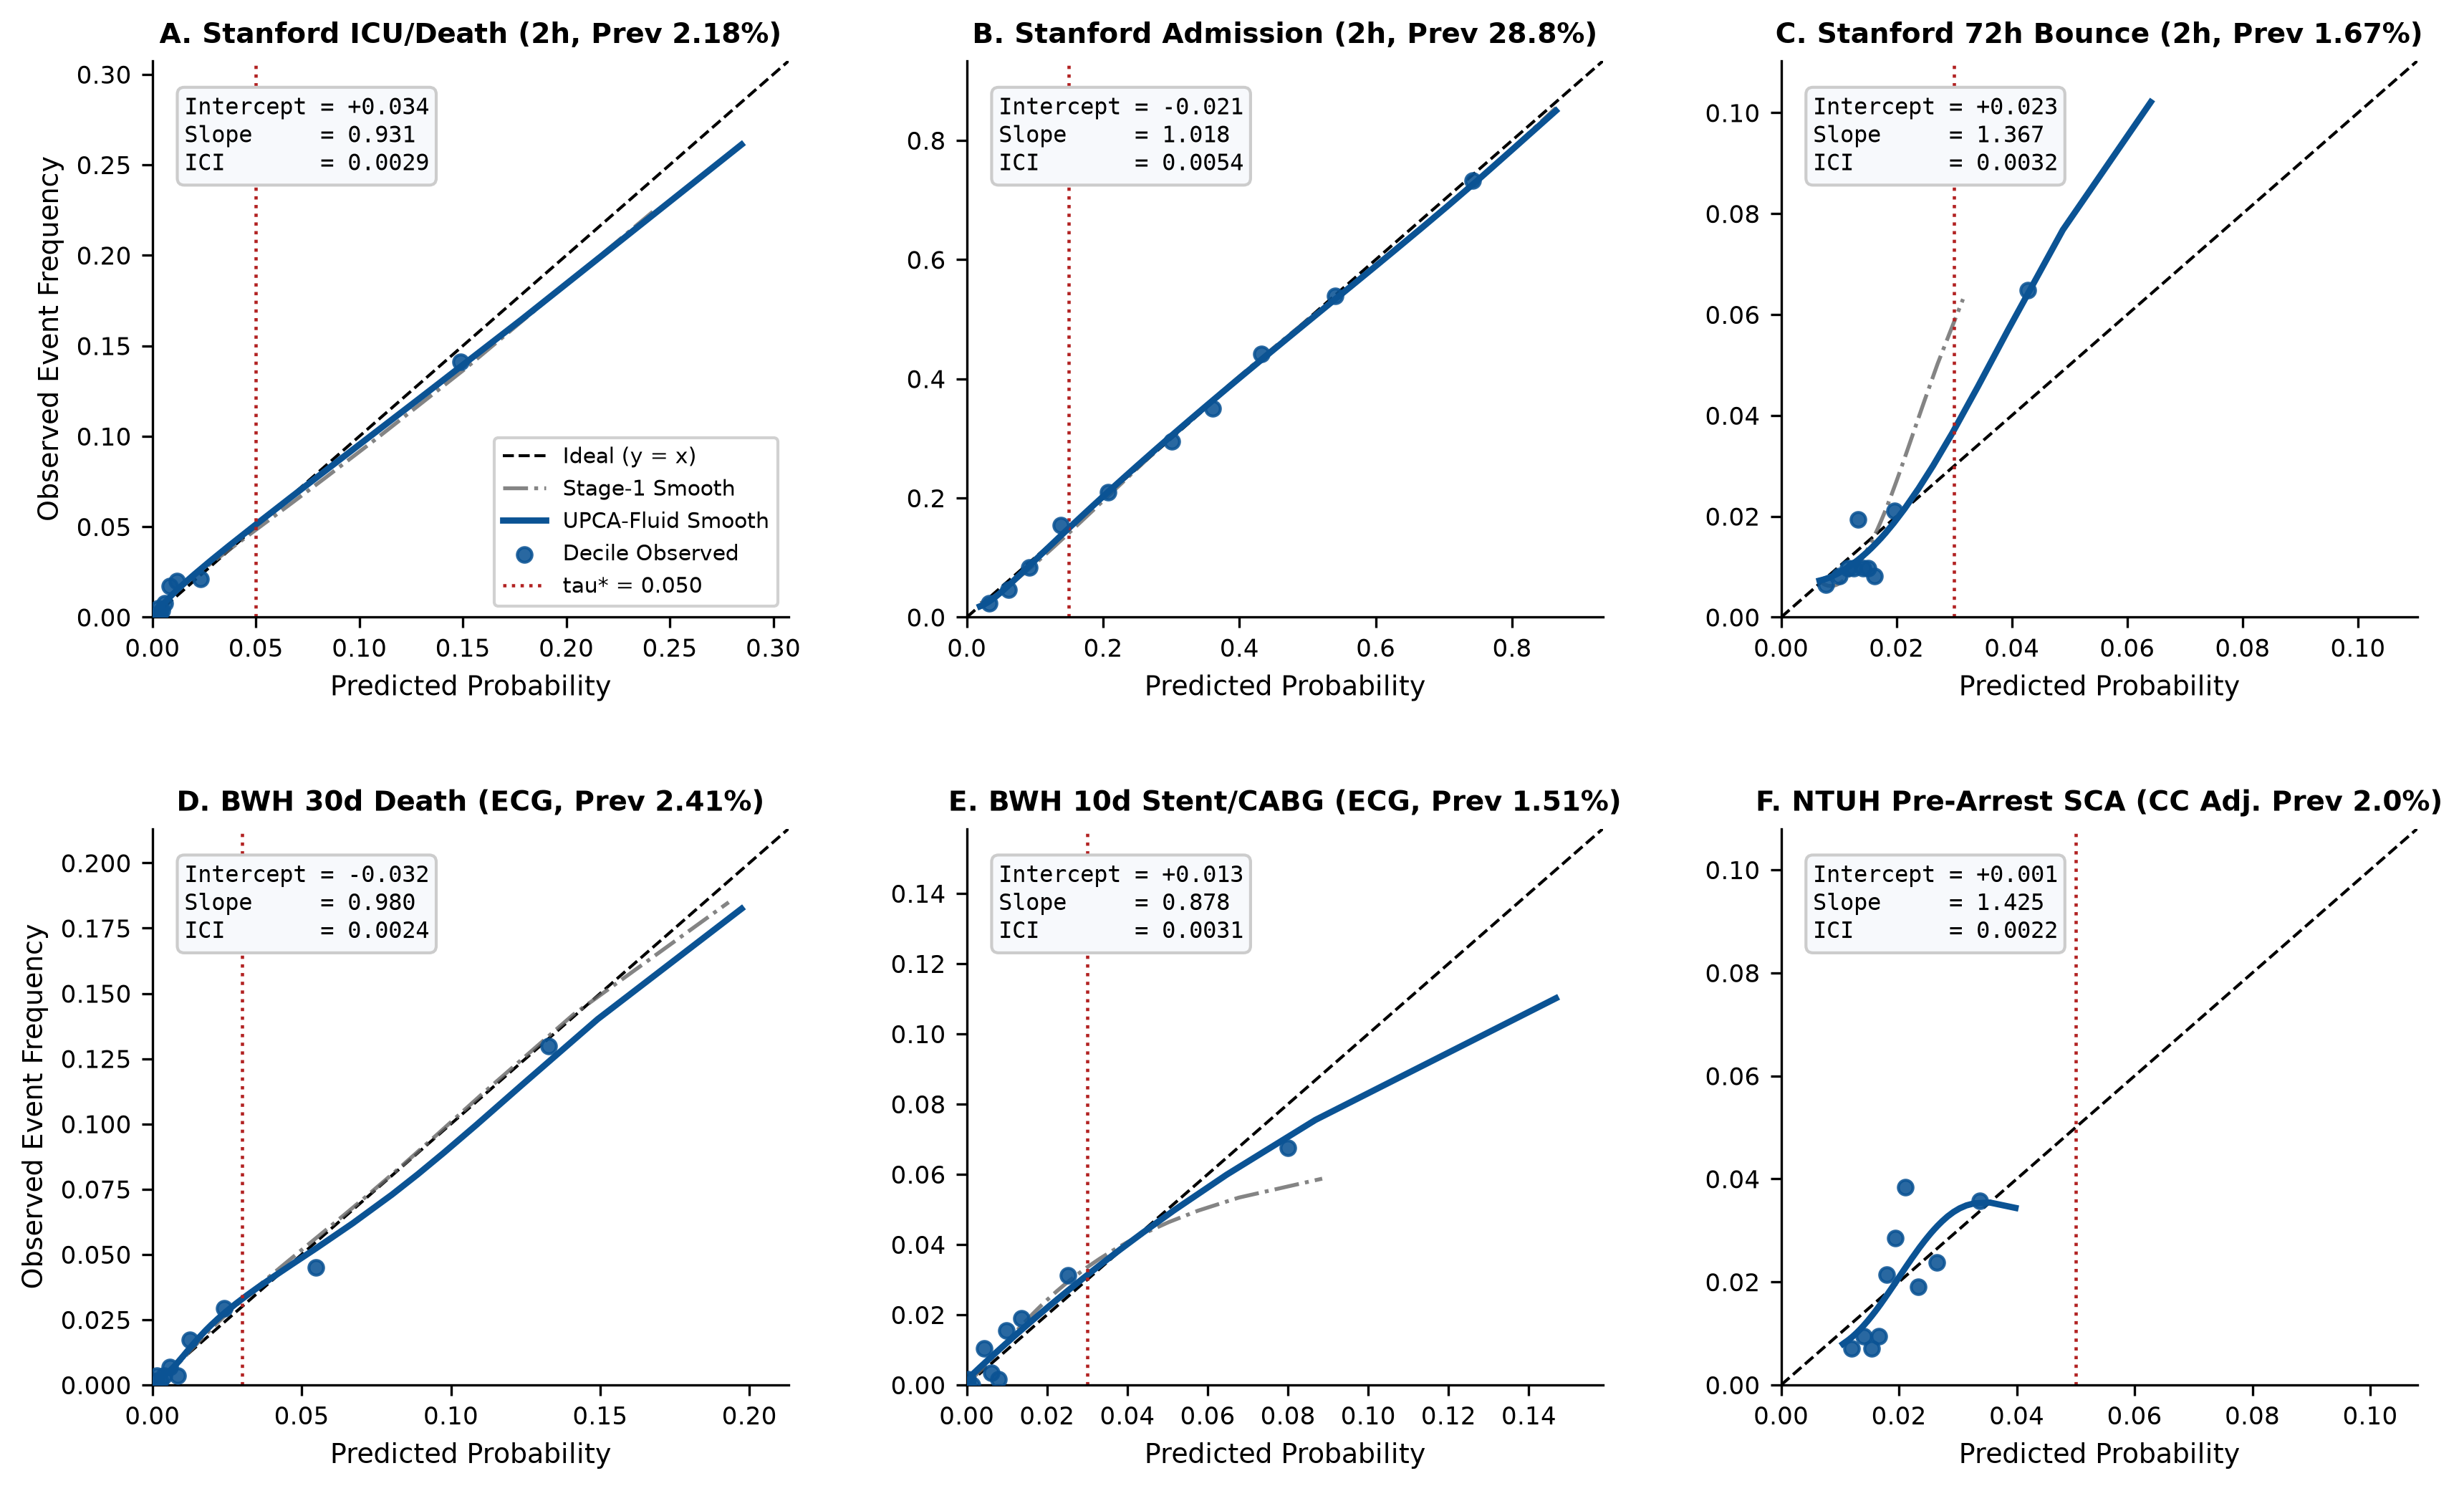
\includegraphics[width=\textwidth]{fig3_calibration_curves.png}
\caption{Flexible spline calibration curves, decile observed event frequencies, calibration-in-the-large ($\text{CITL}$), logistic slope, and Integrated Calibration Index ($\operatorname{ICI}$) across all six primary tasks.}
\label{fig:fig3}
\end{figure}

\textbf{Skipped-Case Bounds, Incorporation/Deconfounding Audits, and Post-Hoc Subgroup Heterogeneity (Table~\ref{tab:governance}, Appendix Table~\ref{tab:subgroup_parity}, Figure~\ref{fig:fig4}):} Under $R=10$ \texttt{Common-Panel Bagged VOI}, patient-cluster $95\%$ upper bounds on skipped-encounter ($Q=0$) action flips remain $\le 0.14\%\text{--}2.82\%$ across all six tasks ($1.11\%$ on Stanford ICU: $71$ beneficial vs.\ $8$ harmful flips among $8{,}485$ skipped encounters; $0.66\%$ on BWH Revascularization). Stripping missingness indicators via \texttt{AgnielDeconfounder} \citep{agniel2018biases} preserves canonical Stanford ICU $\operatorname{NB}=+9.46$ ($+1.09, p=0.0076$) within its linear/homoscedastic scope (Appendix~\ref{app:self_contained}), and BWH \texttt{UPCA-Fluid} achieves $+12.08$ vs.\ $+6.44$ ($p=0.0002$) among $5{,}299$ patients without $10\text{d}$ stress/cath testing while pruning a Stage-A noise channel on complete-troponin $30\text{d}$ mortality ($+13.92\to +14.75$). Auditing $36$ Cochran's $Q$ subgroup heterogeneity tests across \texttt{race}, \texttt{sex}, \texttt{age}, and \texttt{payer}/\texttt{IRS-AGI} against \texttt{Full 100\% All-$M$}, Stage-1, and \texttt{CMI+GBDT} (Appendix Table~\ref{tab:subgroup_parity}) shows \textbf{zero nominal $p_{\text{het}} < 0.05$ flags on primary Stanford ICU ($p_{\text{het}} \in [0.112, 0.897]$ across all $12$ tests)}, whereas \textbf{five post-hoc, hypothesis-generating contrasts reach nominal $p_{\text{het}} < 0.05$} on secondary tasks: (i--iii) on Stanford Admission vs.\ Stage-1 across payer ($Q=15.84, p_{\text{het}}=0.00036$: Medicaid $+8.92$, Commercial $+8.82$ vs.\ Medicare $-5.17$, reflecting $43.3\%$ Medicare base-rate admission already above $\tau^*=0.15$ and $79.6\%$ vs.\ $30.4\%$ CDW medication completeness), age ($Q=6.79, p_{\text{het}}=0.0092$: $<65\text{y}$ $+8.11$ vs.\ $\ge 65\text{y}$ $-0.02$), and sex ($Q=4.43, p_{\text{het}}=0.035$: Female $+8.58$ vs.\ Male $+1.51$); (iv) on Stanford Admission vs.\ \texttt{Full 100\% All-8} by age ($Q=6.67, p_{\text{het}}=0.0098$: $\ge 65\text{y}$ saves $+11.51$ in avoided fees [$q=31.1\%$] vs.\ $+3.94$ for $<65\text{y}$ [$q=65.8\%$]); and (v) on BWH $30\text{d}$ Mortality vs.\ \texttt{CMI+GBDT} by sex ($Q=4.34, p_{\text{het}}=0.037$: Female $+0.60$ vs.\ Male $-1.09$, neither stratum individually significant, $p \ge 0.073$).

\begin{figure}[t]
\centering
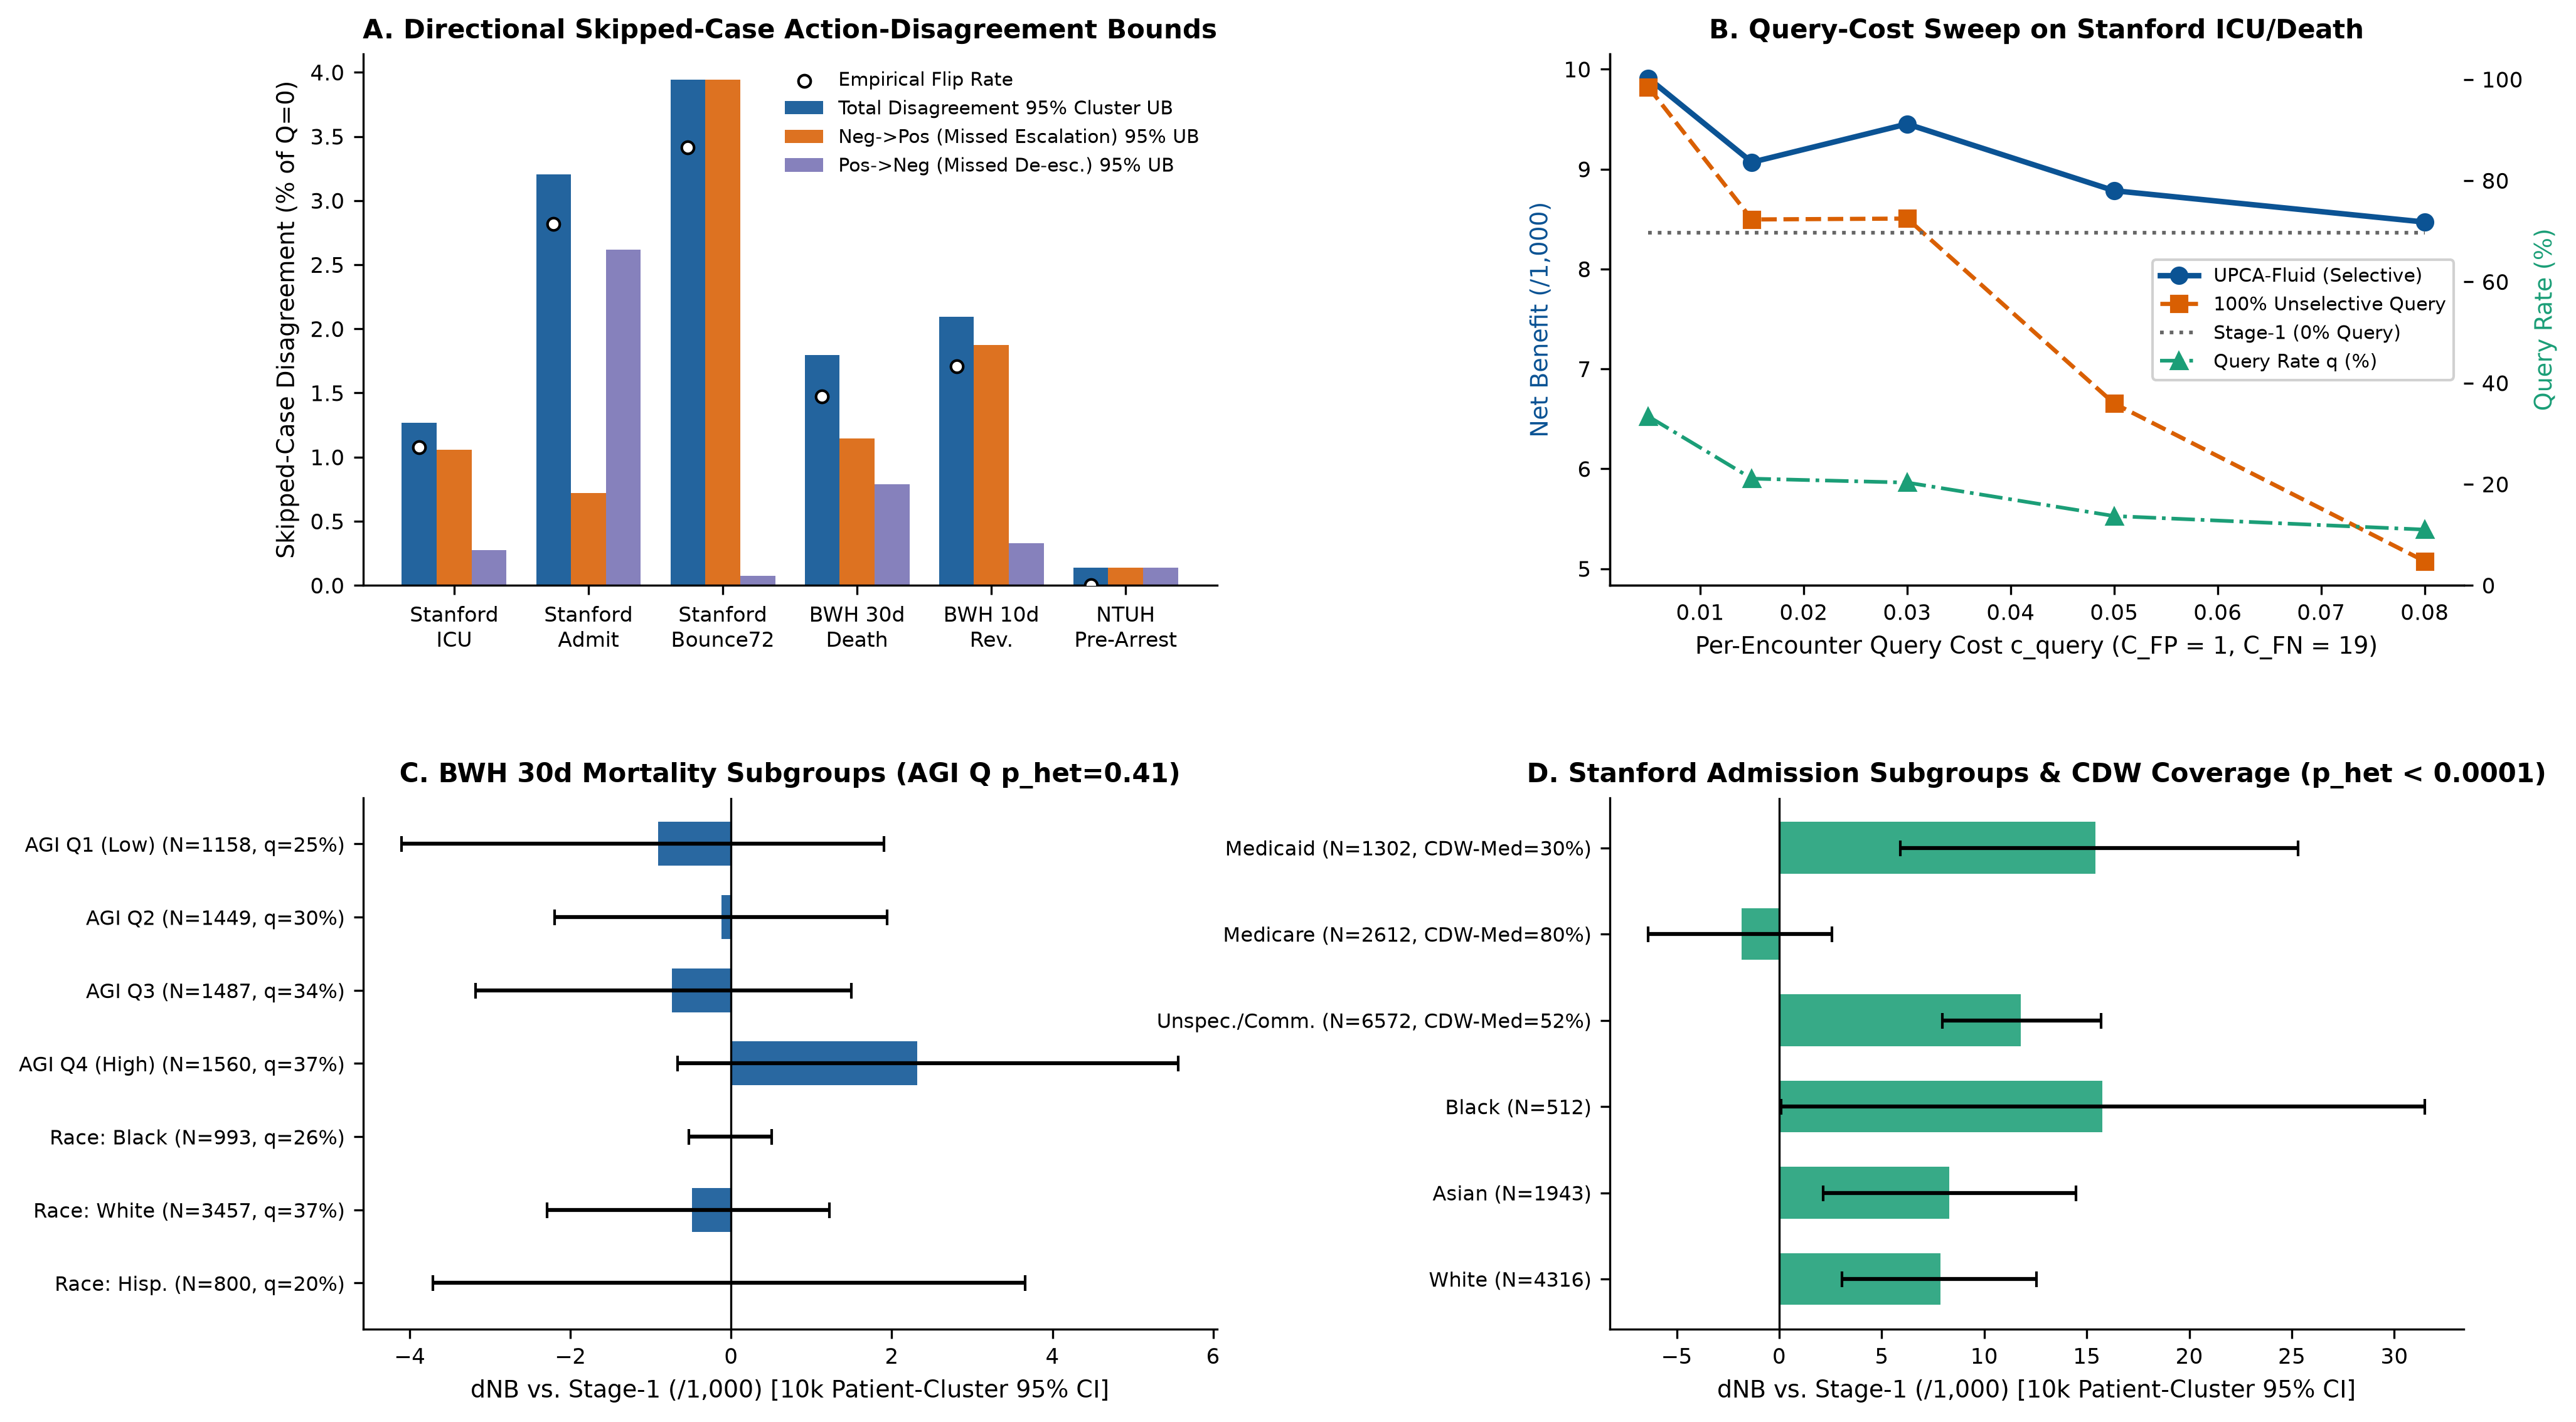
\includegraphics[width=\textwidth]{fig4_skipped_disagreement_and_subgroups.png}
\caption{Directional skipped-case disagreement bounds and multi-comparator subgroup heterogeneity audits ($R=10$ \texttt{Common-Panel Bagged VOI}). \textbf{(A)} Patient-cluster $95\%$ upper bounds on total, $\text{Neg}\to\text{Pos}$, and $\text{Pos}\to\text{Neg}$ action flips among skipped ($Q=0$) test encounters. \textbf{(B--D)} Subgroup $\Delta\operatorname{NB}$ ($10\text{k}$ patient-cluster $95\%$ CIs and Cochran's $Q$ $p_{\text{het}}$) vs.\ \texttt{Full 100\% All-$M$} and vs.\ Stage-1 on Stanford ICU (payer, race) and BWH $30\text{d}$ mortality (IRS ZIP-AGI quartile).}
\label{fig:fig4}
\end{figure}

\begin{table}[t]
\centering
\caption{Skipped-case action-disagreement bounds ($R=10$ \texttt{Common-Panel Bagged VOI}), non-incorporated BWH subgroup evaluations, and process-deconfounding summary ($B=10{,}000$ patient-cluster CIs).}
\label{tab:governance}
\vspace{4pt}
\resizebox{\textwidth}{!}{%
\begin{tabular}{llrrrl}
\toprule
\textbf{Audit Domain} & \textbf{Cohort / Subgroup Slice} & $N_{\text{eval}}$ (\textbf{Events}) & \textbf{Ref.\ $\operatorname{NB}$} & \textbf{\texttt{UPCA} $\operatorname{NB}$} & \textbf{Key Quantitative Finding ($95\%$ Cluster CI / Bound)} \\
\midrule
Skipped Disagreement & Stanford ICU ($Q=0$ Common-Bagged) & 8,485 (143) & --- & --- & Flip $0.93\%$ ($95\%$ UB $1.11\%$: $\text{N}\to\text{P}$ $1.06\%$, $\text{P}\to\text{N}$ $0.08\%$; $71$ ben.\ / $8$ harm.) \\
Skipped Disagreement & BWH 10d Rev.\ ($Q=0$ Common-Bagged) & 3,789 (19) & --- & --- & Flip $0.48\%$ ($95\%$ UB $0.66\%$: $\text{N}\to\text{P}$ $0.66\%$, $\text{P}\to\text{N}$ $0.08\%$; $15$ ben.\ / $3$ harm.) \\
No 10d Stress/Cath & BWH \texttt{test\_010\_day == 0} (30d Death) & 5,299 (125) & $+6.44$ (Tested) & $+12.08$ & $+5.64$ [$+2.90, +8.41$], $p=0.00020$ (flags $96/125$ [$76.8\%$] deaths) \\
No Same-Day Trop.\ & BWH \texttt{trop\_drawn == 0} (30d Death) & 4,104 (81) & $+5.30$ (Tested) & $+9.25$ & $+3.96$ [$+1.02, +6.98$], $p=0.0076$ ($+1.19$ vs.\ S1, $p=0.101$) \\
Complete Troponin & BWH \texttt{trop\_drawn == 1} (10d Rev.) & 1,675 (54) & $+3.42$ (Stage-1) & $+14.17$ & $+10.74$ [$+5.59, +16.27$], $p=0.00040$; $\operatorname{AUPRC}_{\text{full}} 0.080 \to 0.373$ \\
Complete Troponin & BWH \texttt{trop\_drawn == 1} (30d Death) & 1,675 (58) & $+11.66$ (Stage-1) & $+14.75$ & Stage B prunes Stage-A \texttt{ch\_null\_noise\_1} ($+13.92 \to +14.75$ NB) \\
Agniel Deconfound & Stanford ICU (Zero Miss.\ Indicators) & 10,486 (229) & $+8.36$ (Stage-1) & $+9.46$ & $+1.09$ [$+0.27, +1.96$], $p=0.0076$; linear/homoscedastic scope (App.~\ref{app:self_contained}) \\
\bottomrule
\end{tabular}%
}
\end{table}

\section{Discussion and Limitations}
\label{sec:discussion}

Evaluating offset two-phase discovery, channel-scheduled pre-purchase screening, and \texttt{Common-Panel Bagged VOI} across $157{,}324$ unique encounters yields four concrete methodological lessons and operational boundaries:
\begin{enumerate}
  \item \textbf{Pilot Discovery Concordance vs.\ Channel-Scheduled Bedside Net Benefit:} Separating Phase-2 pilot discovery from downstream refitting and billing clarifies what each stage contributes. Across $500$ repeated $20\%$ pilots on Stanford ICU/mortality, unweighted Breslow--Cain offset GBDTs substantially outperform $0.05$-floor downweighting ($87.4\%$ vs.\ $73.8\%$, $p=4.70\times 10^{-12}$) and IPW ($67.6\%$), whereas disjoint $50/50$ split-pilot confirmation guarantees exact finite-sample HT design-unbiasedness ($1.0\%\text{--}1.5\%$ FWER) at a steep $21.0\text{--}43.0$-point power cost. Downstream under \texttt{ChannelCostSchedule}, locking \texttt{[renal\_elyte, lactate\_cardiac]} yields large savings over \texttt{Full 100\% All-8} ($+3.48/1{,}000, p_{\text{DH}}=0.0002$) and \texttt{Full 100\% Locked} ($+1.27, p_{\text{DH}}=0.0004$), while its contrast against zero-query Stage-1 ($+0.12, p_{\text{DH}}=0.758$) is inconclusive and below the $1.0/1{,}000$ reference $\texttt{MCID}$ because pruning \texttt{monitor\_numerics\_2h} trades subtle borderline discrimination for lower panel fees (whereas Admission $+5.35$ and BWH Revascularization $+1.71$ exceed reference $\texttt{MCID}$).
  \item \textbf{Two-Sided Fee Savings vs.\ Sensitivity Preservation via \texttt{Escalation-Only VOI}:} On Stanford ICU, two-sided VOI routing beats \texttt{Full 100\% All-8} Net Benefit across all four thresholds ($+0.99$ to $+7.45/1{,}000$) because fee savings ($+2.38$ to $+8.56$) outweigh small pre-fee losses ($-1.40$ to $-0.58$), but it misses $5\text{--}16$ true critical cases ($-3.7\%\text{ to }-9.1\%$) relative to universal $8$-channel testing, and all net gains depend on the assigned fee schedule ($0.5\times\text{--}3.0\times$ sweep). In high-stakes triage where baseline-flagged patients cannot be de-escalated without full workup, \texttt{Escalation-Only VOI} eliminates baseline sensitivity loss ($0$ missed Stage-1 cases, catching $+7\text{ to }+26$ extra cases) while still querying only $6.3\%\text{--}17.9\%$ of arrivals.
  \item \textbf{Failure of Unlabeled EM Under Rare-Event Overlap and Self-Damping $R_{\text{CZ}}$:} Unlike severe cross-hospital prevalence shifts where disjoint target-site burn-in priors rescue calibration \citep{satz2026collision}, unlabeled \citet{saerens2002adjusting} EM diverges on rare clinical outcomes ($1.5\%\text{--}2.0\%$ prevalence, $\operatorname{NB}=-13.93$ on Bounceback), making disjoint historical calibration priors the safe zero-test-label choice. Similarly, scale-invariant $R_{\text{CZ}} \in [0.000, 0.122]$ shows that on homogeneous clinical panels, KL-gated residual stacking appropriately self-damps to match global GBDTs, while matched-GBDT sequential \texttt{Covert-CMI}/\texttt{Direct-VOI} policies incur $0.05\%\text{--}14.2\%$ null-channel leakage and majority-mask degradation.
  \item \textbf{Limitations:} First, only upstream constants from commit \texttt{8c8c4c8} were fixed pre-\texttt{v1}; \texttt{ChannelCostSchedule}, \texttt{Common-Panel Bagged VOI}, cost sweeps, and the $1.0/1{,}000$ reference $\texttt{MCID}$ are post-\texttt{v1} methodological evaluations. Second, two-sided VOI misses $3.7\%\text{--}9.1\%$ of cases caught by universal $8$-channel querying on Stanford ICU unless \texttt{Escalation-Only VOI} is selected, and Stage-B screening trades $-0.66$ ($-0.92$ flat-fee) under unconstrained $B=2.0$ synthetic budgets and attenuates near $c_{\text{query}}/g \ge 0.90$. Third, post-hoc subgroup heterogeneity emerges on Stanford Admission across payer, age, and sex ($p_{\text{het}} = 0.00036\text{--}0.035$) and on BWH Mortality across sex vs.\ \texttt{CMI+GBDT} ($p_{\text{het}}=0.037$), reflecting base-rate and CDW-completeness gradients that require local subgroup governance \citep{obermeyer2019dissecting,collins2024tripodai}. Fourth, \texttt{Covert-CMI}/\texttt{Direct-VOI} evaluate matched-GBDT policy classes rather than neural DIME, and all clinical benchmarks represent retrospective \emph{in-silico} retrieval of recorded channels requiring prospective silent-mode validation before clinical deployment.
\end{enumerate}

\section*{Author Contributions (CRediT)}

\textbf{Wayne A.\ Satz:} Conceptualization, Methodology, Software, Validation, Formal Analysis, Investigation, Data Curation, Visualization, Writing -- Original Draft, Writing -- Review \& Editing.

\section*{Funding}

This research received no external grant funding. Computational and agentic research platform access was supported in part by the \emph{Google Antigravity for Science} program.

\section*{Institutional Review Board and Informed Consent Statement}

This study was conducted in accordance with the Declaration of Helsinki and Committee on Publication Ethics (COPE) standards for secondary analysis of de-identified research data. New institutional review board approval and informed consent were not applicable because no human participants were recruited, no clinical interventions were performed, no direct identifiers were accessed, and all empirical analyses examine synthetic generators or credentialed, IRB-reviewed, de-identified datasets: \texttt{ed-bwh-ecg} \citep{mullainathan2022diagnosing} and \texttt{arrest-ntuh-ecg/v1} \citep{obermeyer2026ecg} accessed under Nightingale Open Science Data Use Agreements, and \texttt{mcmed-stanford-multi/v1} \citep{kansal2025mcmed} released via Nightingale Open Science and PhysioNet \citep{goldberger2000physionet}. Under U.S.\ federal regulations ($45\text{ CFR }46.102\text{(e)}$), secondary analysis of de-identified datasets does not constitute human subjects research. All results represent retrospective \emph{in-silico} methodological evaluations and are not cleared or validated for clinical patient care.

\section*{Data and Code Availability Statement}

{\raggedright The standalone \texttt{DecisionAwareAcquisition} repository (MIT License; \texttt{LICENSE} and \texttt{CITATION.cff} metadata; preprint archived via \texttt{Preprints.org})---containing \texttt{build\_audited\_cohorts\_v2.py}, \texttt{upca\_v2\_core.py}, \texttt{upca\_v2\_2\_repairs.py}, bundled \texttt{collision\_zone} primitives, \texttt{run\_paper3\_v2\_2\_remediation.py}, $<1\text{s}$ deterministic ledger verifier \texttt{verify\_paper3\_v2\_2\_tables.py}, \texttt{plot\_paper3\_v2\_2\_figures.py}, pinned environment lockfile (\texttt{requirements-lock.txt}), RNG seed ledger (\texttt{SEED\_MANIFEST.md}), automated unit tests ($48/48$ passing \texttt{pytest} tests), and checkpoint JSONs---is publicly archived at \url{https://github.com/deesatzed/DecisionAwareAcquisition/releases/tag/v2.2.0} (immutable computational commit \texttt{9ac6de0}), alongside companion Releases \texttt{v2.2.1} (\url{https://github.com/deesatzed/imboreceipt/releases/tag/v2.2.1}; \citealp{satz2026pilot}) and \texttt{v2.3.1} / commit \texttt{8c8c4c8} (\url{https://github.com/deesatzed/collision-zone-ed/releases/tag/v2.3.1}; \citealp{satz2026collision}). De-identified clinical datasets are accessible to credentialed researchers via Nightingale Open Science (\url{https://ngsci.org}; \citealp{nightingale2024platform}) and PhysioNet (\url{https://physionet.org}; \citealp{kansal2025mcmed,goldberger2000physionet}).\par}

\section*{Competing Interests}

The author declares no competing financial or non-financial interests.

\section*{Acknowledgments}

Computational and agentic research platform access was supported in part by the \emph{Google Antigravity for Science} program. We thank Nightingale Open Science, PhysioNet \citep{goldberger2000physionet}, and the clinical research teams at Brigham and Women's Hospital \citep{mullainathan2022diagnosing}, Stanford University Department of Emergency Medicine \citep{kansal2025mcmed}, and National Taiwan University Hospital \citep{obermeyer2026ecg}, as well as the maintainers of \texttt{LightGBM} \citep{ke2017lightgbm}, \texttt{scikit-learn} \citep{pedregosa2011scikit}, and \texttt{SciPy} \citep{virtanen2020scipy}.

\appendix

\section{Formal Propositions, Null Assumptions, and Mathematical Proofs}
\label{app:proofs}

\begin{proposition}[Mode-Normalized Beta-to-Boltzmann-KL Identity; cf.\ \citealp{schervish1989general,buja2005loss,satz2026collision}]
\label{prop:beta_kl}
For any threshold $\tau^* \in (0,1)$, concentration $\kappa > 0$, and $p \in (0,1)$, let $\alpha_\kappa = 1 + \kappa\tau^*$, $\beta_\kappa = 1 + \kappa(1-\tau^*)$, and $w_{\tau^*,\kappa}(p) = p^{\alpha_\kappa - 1}(1-p)^{\beta_\kappa - 1} / B(\alpha_\kappa, \beta_\kappa)$. Then $w_{\tau^*,\kappa}(p)$ achieves its unique maximum on $(0,1)$ at $p = \tau^*$, and $w_{\tau^*,\kappa}(p)/w_{\tau^*,\kappa}(\tau^*) = \exp(-\kappa D_{\text{KL}}(\operatorname{Bern}(\tau^*)\|\operatorname{Bern}(p)))$ holds identically.
\end{proposition}

\begin{proof}[Proof of Proposition~\ref{prop:beta_kl}]
Substituting $\alpha_\kappa - 1 = \kappa\tau^*$ and $\beta_\kappa - 1 = \kappa(1-\tau^*)$ cancels $B(\alpha_\kappa, \beta_\kappa)$, giving $\log[w_{\tau^*,\kappa}(p)/w_{\tau^*,\kappa}(\tau^*)] = \kappa\tau^*\log(p/\tau^*) + \kappa(1-\tau^*)\log((1-p)/(1-\tau^*)) = -\kappa D_{\text{KL}}(\operatorname{Bern}(\tau^*)\|\operatorname{Bern}(p)) \le 0$, with equality iff $p=\tau^*$.
\end{proof}

\begin{proposition}[Rank-Order Inversion of Routed $\operatorname{AUPRC}$ Under Coherent VOI Skipping]
\label{prop:auprc_inversion}
Let $\eta_1 = \mathbb{P}(Y=1 \mid X_{\text{base}}) \in (0,1)$ and $\eta_2 = \mathbb{P}(Y=1 \mid X_{\text{base}}, Z_{\mathcal{S}}) \in (0,1]$ satisfy $\mathbb{E}[\eta_2 \mid X_{\text{base}}] = \eta_1$ with $\mathbb{P}(Y=1) \in (0,1)$. Suppose there exists $\mathcal{A}_+ = \{x : \eta_1(x) \in [p_{\text{lo}}, p_{\text{hi}}]\} \subset (\tau^*, 1)$ ($\mathbb{P}(X_{\text{base}} \in \mathcal{A}_+) > 0$) with $\mathbb{P}(\eta_2 \ge \tau^* \mid X_{\text{base}} \in \mathcal{A}_+) = 1$, and a queried region $\mathcal{A}_{\text{CZ}}$ ($Q=1$ on $\mathcal{A}_{\text{CZ}}$, $Q=0$ on $\mathcal{A}_+$). Then:
\begin{enumerate}
  \item \emph{Zero Bayes VOI and Strictly Higher Net Benefit:} For $x \in \mathcal{A}_+$, $\operatorname{VOI}(x) = 0$, $\mathbb{I}\{\eta_{\text{route}} \ge \tau^*\} = \mathbb{I}\{\eta_2 \ge \tau^*\} = 1$ almost surely, and skipping $\mathcal{A}_+$ increases $\operatorname{NB}_{\mathcal{K}}$ by $+1000\,(C(\mathcal{S})/C_{\text{FN}})\,\mathbb{P}(X_{\text{base}} \in \mathcal{A}_+) > 0$.
  \item \emph{Strict Global Rank Inversion:} If $\eta_2$ has no point masses on $[p_{\text{lo}}, 1)$, $\mathbb{P}(X_{\text{base}} \in \mathcal{A}_+, \eta_2 > p_{\text{top}}) > 0$ for some $p_{\text{top}} \in (p_{\text{hi}}, 1)$, $\mathbb{P}(X_{\text{base}} \in \mathcal{A}_{\text{CZ}}, Y=0, \eta_2 \in (p_{\text{hi}}, p_{\text{top}})) > 0$, and $\mathbb{P}(\eta_2 > p_{\text{top}}, Y=0) = 0$, then $\operatorname{AUPRC}(\eta_{\text{route}}) < \operatorname{AUPRC}(\eta_2)$ strictly.
\end{enumerate}
\end{proposition}

\begin{proof}[Proof of Proposition~\ref{prop:auprc_inversion}]
\emph{Part 1.} On $\mathcal{A}_+$, $L^*(\eta_1) = (1-\eta_1)C_{\text{FP}}$ and $\eta_2 \ge \tau^*$ a.s.\ implies $\mathbb{E}[L^*(\eta_2)\mid X_{\text{base}}] = \mathbb{E}[(1-\eta_2)C_{\text{FP}}\mid X_{\text{base}}] = L^*(\eta_1)$, so $\operatorname{VOI}=0$ and skipping saves $1000(C(\mathcal{S})/C_{\text{FN}})\mathbb{P}(\mathcal{A}_+)$ with identical threshold decisions. \emph{Part 2.} Under $\eta_2$, thresholds $t > p_{\text{top}}$ have $\operatorname{Prec}_{\eta_2}(t)=1$ on positive recall mass $m_+/\pi > 0$. Under $\eta_{\text{route}}$, $\mathcal{A}_+$ is clamped to $\eta_1 \le p_{\text{hi}} < p_{\text{top}}$ below queried false positives $m_{\text{FP}} = \mathbb{P}(\mathcal{A}_{\text{CZ}}, Y=0, \eta_2 \in (p_{\text{hi}}, p_{\text{top}})) > 0$, forcing $\operatorname{Prec}_{\eta_{\text{route}}}(t) \le \pi/(\pi+m_{\text{FP}}) < 1$ across $[p_{\text{lo}}, p_{\text{hi}}]$ without exceeding $\operatorname{Prec}_{\eta_2}$ elsewhere.
\end{proof}

\begin{proposition}[Skipped-Case Action-Disagreement and Risk-Difference Bounds]
\label{prop:skip_safety}
On skipped test encounters $\mathcal{I}_{\text{skip}} = \{i : Q_i = 0\}$ ($n_{\text{skip}} \ge 1$, $G_{\text{skip}}$ unique patients), let $a_{1,i} = \mathbb{I}\{\hat{p}_{1,i} \ge \tau^*\}$, $a_{2,i} = \mathbb{I}\{\hat{p}_{2,i} \ge \tau^*\}$, and $K_{\text{flip}} = K_{0\to 1} + K_{1\to 0}$. Under independent encounters, one-sided Clopper--Pearson $U_{1-\alpha}^{\text{CP}}(K_\star, n_{\text{skip}})$ \citep{clopper1934use} guarantees coverage $\ge 1-\alpha$ (replaced by patient-cluster bootstrap upper bounds, $1-\alpha^{1/G_{\text{skip}}}$ at $K_\star=0$, under repeat visits), and pre-fee decision risk satisfies $|R_{\text{dec}}(a_{\text{route}}) - R_{\text{dec}}(a_2)| \le \max(C_{\text{FN}}, C_{\text{FP}})\,\mathbb{P}(Q=0)\,p_{\text{flip}}$.
\end{proposition}

\begin{proof}[Proof of Proposition~\ref{prop:skip_safety}]
Binomial coverage follows from the Beta--Binomial identity $\sum_{j=0}^k \binom{n}{j}p_\star^j(1-p_\star)^{n-j} = 1 - I_{p_\star}(k+1,n-k)$ \citep{clopper1934use}. Pointwise loss $\Delta\ell_i = \ell(Y_i, a_{\text{route},i}) - \ell(Y_i, a_{2,i})$ vanishes unless $Q_i=0$ and $a_{1,i}\ne a_{2,i}$, where $|\Delta\ell_i| = C_{\text{FN}}Y_i + C_{\text{FP}}(1-Y_i) \le \max(C_{\text{FN}}, C_{\text{FP}})$; taking expectations yields the bound.
\end{proof}

\begin{proposition}[Population Posterior Recovery Under Offset-Adjusted Two-Phase Sampling]
\label{prop:breslow_cain}
Under stratum-uniform without-replacement sampling $I_i \perp Z_i \mid (Y_i, b_i)$ with $\pi_{\mathcal{P}}(y,b) > 0$, conditional pilot log-odds satisfies Eq.~\eqref{eq:bc_shift} with $\delta_{\mathcal{P}}(b) = \log(\pi_{\mathcal{P}}(1,b)/\pi_{\mathcal{P}}(0,b))$ \citep{breslow1988logistic}, and unweighted ($\text{weight}_i \equiv 1$) Bernoulli cross-entropy minimization of $f_{\mathcal{P}}(x,z) = \operatorname{logit}(\hat{p}_1(x)) + \delta_{\mathcal{P}}(b(x)) + g_{\text{tree}}(x,z)$ on $\mathcal{P}$ has unique population minimizer $\operatorname{logit}(\hat{p}_1(x)) + g_{\text{tree}}^*(x,z) = \operatorname{logit}\mathbb{P}(Y=1 \mid x,z)$.
\end{proposition}

\begin{proof}[Proof of Proposition~\ref{prop:breslow_cain}]
Uniform sampling independent of $Z_{\mathcal{S}}$ gives $\mathbb{P}(I=1 \mid Y=y, x, z) = \pi_{\mathcal{P}}(y,b(x))$, so Bayes' rule yields Eq.~\eqref{eq:bc_shift}. Strict convexity of Bernoulli cross-entropy gives unique pointwise minimizer $f_{\mathcal{P}}^*(x,z) = \operatorname{logit}\mathbb{P}(Y=1\mid x,z,I=1) = \operatorname{logit}\mathbb{P}(Y=1\mid x,z) + \delta_{\mathcal{P}}(b(x))$.
\end{proof}

\begin{assumption}[Learner-Specific Predictive-Utility Null and Disjoint Split Confirmation]
\label{assump:learner_null}
For step-level baseline predictor $\hat{p}_{\text{base}}$ and Stage-A learner family $\mathcal{G}$, a candidate channel $m$ satisfies the \emph{learner-specific predictive-utility null} if $\mathbb{E}[S_{\tau^*,\kappa_{\text{eff}}}(Y, \hat{p}_{\text{aug}}) - S_{\tau^*,\kappa_{\text{eff}}}(Y, \hat{p}_{\text{base}})] \le 0$. Under disjoint $50/50$ split-pilot confirmation ($\mathcal{P} = \mathcal{P}_{\text{fit}} \sqcup \mathcal{P}_{\text{eval}}$), conditional on $\mathcal{P}_{\text{fit}}$, score differences $\{u_i\}_{i \in \mathcal{P}_{\text{eval}}}$ are fixed functions of Phase-2 observations, so $\hat{\Delta}_{\text{eval}}$ is exactly Horvitz--Thompson design-unbiased with variance estimated by Eq.~\eqref{eq:twophase_var}.
\end{assumption}

\begin{remark}[Analytic Finite-Capacity \texttt{XOR} Counterexample]
\label{rem:xor_null}
Population conditional independence $I(Y; Z \mid X_{\text{base}}) = 0$ does not imply $\mathbb{E}[\Delta S] \le 0$ under a finite-capacity Stage-1 model: let $X_1, X_2 \in \{\pm 1\}$ be independent Rademacher variables, $Y = \mathbb{I}\{X_1 X_2 = 1\}$ (or prevalence-shifted XOR), and $Z = X_1 X_2 + \varepsilon$ ($I(Y;Z\mid X_1,X_2)=0$). A depth-$1$ stump Stage-1 learner cannot represent $X_1 X_2$, whereas adding $Z$ yields strictly positive Schervish score gain ($+0.14108$) and log-loss gain ($+0.68685$ at $N=2{,}400$; verified in \texttt{xor\_\allowbreak finite\_\allowbreak capacity\_\allowbreak counterexample}). Stage-A FWER guarantees therefore govern Assumption~\ref{assump:learner_null} rather than learner-free conditional independence.
\end{remark}

\begin{proposition}[Population Pre-Purchase Identifiability Separation and Subset FWER Preservation]
\label{prop:prepurchase}
Suppose collision-zone encounters ($\eta_1(X_{\text{base}})=\tau^*$, mass $\pi_{\text{CZ}}>0$) carry $U_{\text{id}}, U_{\text{unid}} \sim \operatorname{Bern}(\rho)$ where $U_{\text{id}}$ is $X_{\text{base}}$-measurable, $(U_{\text{unid}}, Z_{m_{\text{unid}}}) \perp X_{\text{base}} \mid \eta_1(X_{\text{base}})$, and active status induces point-$\tau^*$ Bayes VOI $g > 0$ ($\eta_2=\eta_1$ otherwise). Whenever $\rho g < C(\{m\}) < g$, both channels have identical post-purchase CMI and Beta-KL gains, yet $\Delta V^*(m_{\text{id}}) = \pi_{\text{CZ}}\rho(g - C(\{m_{\text{id}}\})) > 0$ while $\Delta V^*(m_{\text{unid}}) = 0$; furthermore, any $\hat{\mathcal{S}}_{\text{UPCA}} \subseteq \mathcal{C}_{\text{Holm}}$ preserves $\mathbb{P}(\hat{\mathcal{S}}_{\text{UPCA}} \cap \mathcal{H}_0 \ne \emptyset) \le \alpha$.
\end{proposition}

\begin{proof}[Proof of Proposition~\ref{prop:prepurchase}]
Identical conditional laws given $\eta_1$ yield equal post-purchase gains. Measurability of $U_{\text{id}}$ gives $\operatorname{VOI}(X_{\text{base}}) = g > C(\{m_{\text{id}}\})$ on mass $\pi_{\text{CZ}}\rho$, whereas $(U_{\text{unid}}, Z_{m_{\text{unid}}}) \perp X_{\text{base}} \mid \eta_1$ averages pre-purchase VOI to $\rho g < C(\{m_{\text{unid}}\})$, maximized at $Q \equiv 0$. Monotonicity $\hat{\mathcal{S}}_{\text{UPCA}} \subseteq \mathcal{C}_{\text{Holm}}$ preserves FWER $\le \alpha$.
\end{proof}

\section{Self-Contained Algorithmic Specifications}
\label{app:self_contained}

\begin{enumerate}
  \item \textbf{Mode-Aligned Beta Score and Neyman Pilot Allocation \citep{schervish1989general,buja2005loss,tao2020optimal}:} With $\alpha_\kappa = 1+\kappa\tau^*$ and $\beta_\kappa = 1+\kappa(1-\tau^*)$,
  \begin{equation}
    S_{\tau^*,\kappa}(y, p) = -y\,\frac{\beta_\kappa}{\alpha_\kappa+\beta_\kappa}\big(1 - I_p(\alpha_\kappa, \beta_\kappa+1)\big) - (1-y)\,\frac{\alpha_\kappa}{\alpha_\kappa+\beta_\kappa}\, I_p(\alpha_\kappa+1, \beta_\kappa),
    \label{eq:schervish_app}
  \end{equation}
  and stratum $h=(y,b)$ receives Neyman dispersion weight
  \begin{equation}
    d_h = w_{\tau^*,\kappa}(\bar{p}_h)\,\bar{p}_h(1-\bar{p}_h)\big(|\bar{y}_h - \bar{p}_h| + 0.15\big) + 10^{-3},
    \label{eq:neyman_disp}
  \end{equation}
  allocated via water-filling $n_h \propto N_h d_h$ subject to $2 \le n_h \le N_h$ and $\sum_h n_h = n_{\text{pilot}}$. Dynamic KL-ESS (\texttt{solve\_ess\_kappa}) solves $\sum_{i=1}^n \exp(-2\kappa_{\text{eff}} d_i) = M_{\min}$ ($\max(160, 0.24n)$ in pilots; $240$ in Stage-2).
  \item \textbf{Leak-Free Encoding and KL-Gated Stage-2 Residual Backbone:} \texttt{FastFrameEncoder} imputes training medians + missingness indicators on numeric columns and top-$64$ codes on categoricals strictly inside training folds. \texttt{FluidCollisionBackboneClassifier} stacks unweighted global GBDT $f_{\text{glob}}$ ($140$ trees, $31$ leaves, Platt-calibrated; \citealp{platt1999probabilistic}) with KL-gated residual GBDT $\Delta_{\text{CZ}}$ ($\pi_{\text{union},i} = 1 - (1 - e^{-\kappa^* d(\sigma(\ell_{1,i}))})(1 - e^{-\kappa^* d(\sigma(f_{\text{glob},i}))})$) via $3$-fold OOF L-BFGS-B optimization of $-S_{\tau^*,20}(Y,\sigma(f)) - 0.05\ell_{\log}(Y,\sigma(f)) + 2\times 10^{-4}[(\beta_{\text{glob}}-1)^2 + \beta_{\text{CZ}}^2 + \alpha_0^2]$:
  \begin{equation}
    f(x, z) = \alpha_0 + \beta_{\text{glob}}\,f_{\text{glob}}(x, z) + \beta_{\text{CZ}}\,\pi_{\text{union}}\big(\ell_1(x), f_{\text{glob}}(x,z)\big)\,\Delta_{\text{CZ}}\big(\ell_1(x), f_{\text{glob}}(x,z), z\big).
    \label{eq:fluid_backbone_app}
  \end{equation}
  \item \textbf{Empirical Martingale VOI and Unlabeled Saerens EM:} Damped Newton--Raphson solves for $\mu_i^* \in \mathbb{R}$ satisfying
  \begin{equation}
    \frac{1}{K}\sum_{r=1}^{K} \sigma\!\big(\operatorname{logit}(p_{1,i}) + \mu_i^* + \delta_{c(i),r}\big) = p_{1,i}, \quad \widehat{\operatorname{VOI}}_i = \max\!\left\{0,\, L^*(p_{1,i}) - \frac{1}{K}\sum_{r=1}^{K} L^*(\tilde{p}_{2,i,r})\right\},
    \label{eq:emp_voi_app}
  \end{equation}
  with $\tilde{p}_{2,i,r} = \sigma(\operatorname{logit}(p_{1,i}) + \mu_i^* + \delta_{c(i),r})$. In Table~\ref{tab:prior_shift}, \citet{saerens2002adjusting} EM iterates $\pi^{(t+1)} = N_{\text{test}}^{-1}\sum_i \frac{(\pi^{(t)}/\pi_0)p_i}{(\pi^{(t)}/\pi_0)p_i + ((1-\pi^{(t)})/(1-\pi_0))(1-p_i)}$ solely on unlabeled test predictions $\{p_i\}$ without accessing $Y_{\text{test}}$.
  \item \textbf{Null-Calibrated Process Deconfounder Scope (\texttt{AgnielDeconfounder}):} Ridge regression ($\alpha=10$) fits $\hat{\mu}_c(X_{\text{base}})$ and empirical residuals on measured training rows ($D_c=1$), replacing unmeasured entries with $\hat{\mu}_c(X_{\text{base},i}) + \varepsilon_{c,i}^*$ and suppressing missingness indicators. This removes clinician-ordering indicators under biological nullity ($Y \perp Z_c \mid X_{\text{base}}, D_c=1$; \citealp{agniel2018biases}) up to linear-mean, homoscedastic-residual approximation limits, and does not constitute causal transport under unmeasured confounding \citep{vonkleist2025evaluation}.
\end{enumerate}

\section{Supplementary Tables: Estimand Audit, Pilot Efficiency, Sensitivity, and Subgroup Heterogeneity}
\label{app:supplement}

\begin{table}[h!]
\centering
\caption{Complete Estimand Audit under \texttt{ChannelCostSchedule}: Canonical Single-Split, $R=10$ \texttt{Common-Panel Bagged VOI}, \texttt{Union-Panel} (Rerouted vs.\ Fixed-$q$ Billed vs.\ Legacy Flat-Unbilled), Fractionally Billed \texttt{Sym.\ Ens.}, \texttt{Per-Split} Mean $\pm$ SE, $50/50$ Split-Pilot \texttt{UPCA}, and NTUH \texttt{[1]ROSC}.}
\label{tab:estimands_supp}
\vspace{4pt}
\resizebox{\textwidth}{!}{%
\begin{tabular}{lcccccccc}
\toprule
\textbf{Cohort \& Task} & \textbf{Canon.\ S1 / Full-All} & \textbf{Canon.\ \texttt{UPCA} ($\Delta$ S1, $p$)} & \textbf{$50/50$ Split \texttt{UPCA}} & \textbf{Common-Bagged \texttt{UPCA}} & \textbf{Union Rerouted ($C_{\text{union}}$)} & \textbf{Union Fixed-$q$ / Legacy} & \textbf{\texttt{Sym.\ Ens.}} & \textbf{\texttt{Per-Split} $\pm$ SE} \\
\midrule
1.\ Stanf.\ ICU ($10{,}486$) & $+8.36 / +5.38$ & $+8.97$ ($+0.61, .200$) & $+8.79$ ($.020$) & $\mathbf{+9.00}$ ($.031$) & $+9.18$ ($.048$) & $+9.12 / +9.30$ & $+9.48$ & $+8.99 \pm 0.07$ \\
2.\ Stanf.\ Admit ($10{,}486$) & $+187.12 / +190.54$ & $+196.03$ ($\mathbf{+8.91, .0002}$) & $+195.01$ ($.026$) & $\mathbf{+195.09}$ ($.026$) & $+196.73$ ($.041$) & $+196.55 / +198.09$ & $+197.59$ & $+195.43 \pm 0.29$ \\
3.\ Stanf.\ Bounce ($6{,}165$) & $+0.56 / +2.45$ & $+3.19$ ($\mathbf{+2.63, .0026}$) & $+2.91$ ($.010$) & $\mathbf{+2.91}$ ($.010$) & $+3.32$ ($.030$) & $+3.39 / +3.47$ & $+3.55$ & $+3.34 \pm 0.12$ \\
4.\ BWH 30d Death ($5{,}779$) & $+11.40 / +11.61$ & $+11.84$ ($+0.43, .530$) & $+12.02$ ($.016$) & $\mathbf{+12.02}$ ($.016$) & $+11.93$ ($.016$) & $+11.94 / +11.91$ & $+11.83$ & $+11.34 \pm 0.13$ \\
5.\ BWH 10d Rev.\ ($5{,}779$) & $+2.93 / +4.02$ & $+3.92$ ($+0.99, .225$) & $+4.84$ ($.010$) & $\mathbf{+4.84}$ ($.010$) & $+4.77$ ($.015$) & $+4.78 / +4.73$ & $+4.62$ & $+3.80 \pm 0.20$ \\
6.\ NTUH Pre-Arrest ($3{,}651$) & $-0.04 / -1.74$ & $-0.04$ ($+0.00, 1.00$) & $+0.18$ ($.000$) & $\mathbf{+0.18}$ ($.000$) & $+0.18$ ($.012$) & $+0.18 / +0.18$ & $+0.19$ & $-0.06 \pm 0.06$ \\
\midrule
S1.\ NTUH \texttt{[1]ROSC} Surv./CPC ($130$) & $+288.5 / +242.6$ & $+288.5 / +242.6$ (tie) & --- & $+311.5 / +241.7^*$ & --- & --- & --- & --- \\
\bottomrule
\multicolumn{9}{l}{\footnotesize $^*$Evaluated across $R=5$ patient-grouped splits on \texttt{[1]ROSC} ($+311.54$ exact tie on Survival; $+241.66$ vs.\ $+241.53$ \texttt{WCZ}, $p_{\text{DH}}=0.0132$ on CPC 1--2).}
\end{tabular}%
}
\end{table}

\begin{table}[h!]
\centering
\caption{Within-Stratum Pilot Independence ($I_i \perp Z_i \mid Y_i, b_i$), $500$-Pilot Efficiency (\citealp{breslow1988logistic,tao2017efficient}), $200$-Pilot Split Confirmation, and Constant Sensitivity.}
\label{tab:r15_supp}
\vspace{4pt}
\resizebox{\textwidth}{!}{%
\begin{tabular}{lccccl}
\toprule
\textbf{Primary Clinical Task} & \textbf{Feat.} & \textbf{Med.\ $p$} & \textbf{Mahalanobis $\chi^2$ ($\text{df}$)} & \textbf{Omnibus $p$} & \textbf{Repeated-Pilot Efficiency, Split-Pilot Power, \& Constant Sensitivity Summary} \\
\midrule
1.\ Stanford ICU/Death & 72 & $0.366$ & $70.21$ ($72$ std.) & $0.538$ (perm.\ $.517$) & $500$-Pilot Top-1: WCZ $73.8\%$, IPW $67.6\%$, \textbf{Offset $87.4\%$ ($p=4.7\times 10^{-12}$)} \\
2.\ Stanford Admission & 72 & $0.485$ & $26.34$ ($22$) & $0.237$ & $150$-Pilot \texttt{mon} Bundle: WCZ $88.0\%$, IPW $78.7\%$, \textbf{Offset $98.0\%$ ($p=2.8\times 10^{-4}$)} \\
3.\ Stanford 72h Bounce & 72 & $0.442$ & $17.45$ ($29$) & $0.955$ & $200$-Pilot ($\rho=0.20$ + $2$ Nulls): \textbf{4-Fold CF $82.0\%$ (FWER $0.0\%$)} vs.\ \textbf{50/50 Split $61.0\%$ (FWER $1.0\%$)} \\
4.\ BWH 30d Mortality & 70 & $0.544$ & $61.67$ ($64$) & $0.559$ & $\rho_{\text{pilot}}=0.15 / 0.30$ ($200$ pilots): \textbf{$74.0\%$ vs.\ $61.0\%$} ($p=1.6\times 10^{-4}$) / \textbf{$100.0\%$ vs.\ $96.5\%$} ($p=.0156$) \\
5.\ BWH 10d Stent/CABG & 70 & $0.483$ & $67.57$ ($63$) & $0.324$ & Parametric Lactate Slope RMSE ($500$ pilots): IPW $0.01876$ vs.\ \textbf{Offset MLE $0.01519$ ($-34.5\%$ var.)} \\
6.\ NTUH Pre-Arrest SCA & 82 & $0.538$ & $42.06$ ($58$) & $0.943$ & Constant grid ($B_{\text{score}}\in\{6,12\}, q_{\text{disp}}\in\{.65,.85\}, \alpha_{\text{pol}}\in\{.05,.20\}$): ICU $+8.98\text{--}+9.45$, Rev.\ $+3.88\text{--}+4.34$ \\
\bottomrule
\end{tabular}%
}
\end{table}

\begin{table}[h!]
\centering
\caption{Multi-Comparator Subgroup Equity, Calibration (\texttt{CITL}, Slope, \texttt{ICI}), Error-Rate Parity (\texttt{FNR}, \texttt{FPR}), and Cochran's $Q$ Heterogeneity Audit ($R=10$ \texttt{Common-Panel Bagged VOI}, $B=10{,}000$ patient-cluster bootstraps; all $5$ nominal $p_{\text{het}}<0.05$ contrasts across $36$ tests flagged with $^\dagger$).}
\label{tab:subgroup_parity}
\vspace{4pt}
\resizebox{\textwidth}{!}{%
\begin{tabular}{llrrrccccc}
\toprule
\textbf{Task \& Cochran's $Q$ ($p_{\text{het}}$: All / S1 / CMI)} & \textbf{Subgroup Stratum} & $N_{\text{enc}}$ & \textbf{Prev.} & \textbf{$q\%$} & \textbf{$\Delta\operatorname{NB}$ vs.\ Full-All} & \textbf{$\Delta\operatorname{NB}$ vs.\ S1} & \textbf{$\Delta\operatorname{NB}$ vs.\ CMI} & \textbf{\texttt{CITL} / Slope / \texttt{ICI}} & \textbf{$\text{FNR}_{\tau^*} / \text{FPR}_{\tau^*}$} \\
\midrule
\multirow{5}{*}{\shortstack[l]{Stanford ICU: Payer ($.897 / .246 / .352$)\\\& Age ($.476 / .839 / .373$)\\(Race $p_{\text{het}}: .612 / .413 / .192$;\\Sex $p_{\text{het}}: .112 / .863 / .872$)}}
  & Medicaid & 1,302 & $1.61\%$ & $13.3\%$ & $+3.30$ [$-0.58,+6.88$] & $-0.78$ [$-3.54,+1.79$] & $+0.80$ [$-1.66,+3.63$] & $+.06 / 0.98 / .0051$ & $42.9\% / 5.5\%$ \\
  & Medicare & 2,612 & $3.33\%$ & $31.9\%$ & $+3.79$ [$+2.41,+5.26$] & $-0.86$ [$-2.87,+1.00$] & $-0.60$ [$-1.04,-0.18$] & $-.22 / 0.93 / .0093$ & $29.9\% / 17.7\%$ \\
  & Comm.\ / Unspec. & 6,572 & $1.84\%$ & $15.2\%$ & $+3.39$ [$+2.36,+4.38$] & $+0.69$ [$-0.14,+1.61$] & $-0.07$ [$-0.94,+0.81$] & $-.04 / 1.00 / .0023$ & $38.0\% / 6.8\%$ \\
  & Age $<65\text{y}$ & 6,927 & $1.44\%$ & $12.8\%$ & $+3.24$ [$+2.18,+4.20$] & $+0.05$ [$-0.69,+0.79$] & $-0.30$ [$-1.15,+0.51$] & $-.06 / 0.97 / .0022$ & $46.0\% / 5.0\%$ \\
  & Age $\ge 65\text{y}$ & 3,559 & $3.63\%$ & $31.4\%$ & $+3.93$ [$+2.35,+5.57$] & $+0.26$ [$-1.58,+2.13$] & $+0.30$ [$-0.58,+1.45$] & $-.13 / 0.97 / .0073$ & $27.1\% / 17.9\%$ \\
\midrule
\multirow{7}{*}{\shortstack[l]{Stanford Admission:\\Payer ($.394 / \mathbf{.00036}^\dagger / .961$),\\Age ($\mathbf{.0098}^\dagger / \mathbf{.0092}^\dagger / .734$),\\Sex ($.801 / \mathbf{.0353}^\dagger / .416$)\\(Race $p_{\text{het}}: .341 / .452 / .189$)}}
  & Medicaid (Med $30\%$) & 1,302 & $26.1\%$ & $64.8\%$ & $+4.81$ [$-3.05,+12.9$] & $+8.92$ [$-1.35,+19.1$] & $+1.61$ [$-6.93,+10.1$] & $+.41 / 1.02 / .0596$ & $17.4\% / 30.0\%$ \\
  & Medicare (Med $80\%$) & 2,612 & $43.3\%$ & $32.7\%$ & $+9.75$ [$+4.46,+15.2$] & $-5.17$ [$-11.0,+0.26$] & $+0.51$ [$-3.54,+4.64$] & $+.22 / 0.95 / .0437$ & $4.8\% / 79.2\%$ \\
  & Comm.\ / Unspec. & 6,572 & $23.5\%$ & $60.4\%$ & $+5.55$ [$+2.06,+9.08$] & $+8.82$ [$+4.43,+13.1$] & $+1.14$ [$-2.37,+4.66$] & $+.07 / 1.06 / .0115$ & $15.1\% / 38.4\%$ \\
  & Age $<65\text{y}$ & 6,927 & $21.9\%$ & $65.8\%$ & $+3.94$ [$+0.59,+7.35$] & $+8.11$ [$+3.64,+12.5$] & $+0.75$ [$-2.75,+4.28$] & $+.15 / 1.04 / .0203$ & $19.5\% / 32.3\%$ \\
  & Age $\ge 65\text{y}$ & 3,559 & $42.1\%$ & $31.1\%$ & $+11.51$ [$+7.01,+16.2$] & $-0.02$ [$-4.41,+4.09$] & $+1.62$ [$-1.99,+5.19$] & $+.16 / 1.02 / .0318$ & $3.3\% / 79.8\%$ \\
  & Female & 5,686 & $25.4\%$ & $57.4\%$ & $+6.18$ [$+2.34,+10.0$] & $+8.58$ [$+4.07,+13.1$] & $+2.04$ [$-1.63,+5.71$] & $+.10 / 1.05 / .0166$ & $13.5\% / 40.6\%$ \\
  & Male & 4,800 & $32.8\%$ & $50.1\%$ & $+6.89$ [$+2.86,+10.7$] & $+1.51$ [$-3.34,+6.32$] & $-0.14$ [$-3.87,+3.58$] & $+.21 / 1.00 / .0336$ & $9.7\% / 51.7\%$ \\
\midrule
\multirow{6}{*}{\shortstack[l]{BWH 30d Mortality:\\IRS-AGI ($.358 / .698 / .250$),\\Sex ($.295 / .914 / \mathbf{.0373}^\dagger$)\\(Race $p_{\text{het}}: .258 / .614 / .545$;\\Age $p_{\text{het}}: .876 / .393 / .339$)}}
  & Q1 Lowest Income & 1,158 & $1.55\%$ & $25.7\%$ & $+0.54$ [$+0.31,+0.75$] & $+0.79$ [$-0.33,+2.74$] & $-0.05$ [$-0.24,+0.14$] & $+.20 / 1.31 / .0028$ & $33.3\% / 10.2\%$ \\
  & Q2 Low--Mid & 1,449 & $2.55\%$ & $32.0\%$ & $-0.81$ [$-2.96,+0.69$] & $+0.19$ [$-3.13,+3.54$] & $-1.27$ [$-3.42,+0.17$] & $+.36 / 1.01 / .0078$ & $32.4\% / 15.0\%$ \\
  & Q3 High--Mid & 1,487 & $2.09\%$ & $36.5\%$ & $+0.72$ [$+0.46,+0.98$] & $+0.53$ [$-1.46,+2.53$] & $-0.61$ [$-2.07,+0.21$] & $-.02 / 0.94 / .0047$ & $35.5\% / 18.9\%$ \\
  & Q4 Highest Income & 1,560 & $3.01\%$ & $39.0\%$ & $+0.51$ [$-1.42,+2.39$] & $+2.57$ [$-0.39,+5.92$] & $+1.20$ [$-0.16,+3.18$] & $+.30 / 1.26 / .0072$ & $21.3\% / 20.0\%$ \\
  & Female & 3,172 & $2.21\%$ & $31.8\%$ & $+0.60$ [$-0.33,+1.52$] & $+1.00$ [$-0.36,+2.50$] & $+0.60$ [$-0.09,+1.60$] & $+.21 / 1.17 / .0044$ & $25.7\% / 15.5\%$ \\
  & Male & 2,607 & $2.65\%$ & $36.2\%$ & $-0.15$ [$-1.39,+0.71$] & $+1.16$ [$-1.44,+3.87$] & $-1.09$ [$-2.62,+0.05$] & $+.26 / 1.06 / .0061$ & $31.9\% / 17.5\%$ \\
\bottomrule
\end{tabular}%
}
\end{table}

\section{Version \texttt{v2.2.0} Methodological Revision Ledger}
\label{app:ledger}

To ensure transparent auditability across companion revisions \citep{satz2026pilot,satz2026collision}, Table~\ref{tab:rev_ledger} records every methodological, cost-accounting, and reporting update from \texttt{v2.1} to \texttt{v2.2.0} (verified in $<1\text{s}$ via \texttt{scripts/verify\_paper3\_v2\_2\_tables.py} at commit \texttt{9ac6de0}).

\begin{table}[h!]
\centering
\caption{Methodological and clinical-governance revision ledger for \texttt{v2.2.0} (code commit \texttt{9ac6de0}).}
\label{tab:rev_ledger}
\scriptsize
\renewcommand{\arraystretch}{1.12}
\begin{tabular}{>{\raggedright\arraybackslash}p{0.21\textwidth}>{\raggedright\arraybackslash}p{0.34\textwidth}>{\raggedright\arraybackslash}p{0.37\textwidth}}
\toprule
\textbf{Audit Dimension} & \textbf{Prior \texttt{v2.1} State / Vulnerability} & \textbf{\texttt{v2.2.0} Resolution \& Empirical Impact} \\
\midrule
1.\ Literature Credit \& Beta-KL / HT Variance Identities & Credited \citet{schervish1989general} without \citet{buja2005loss}, \citet{turney1995cost}, \citet{bilgic2011value}, or \citet{saerens2002adjusting}; omitted explicit two-phase HT variance formula and \texttt{XOR} finite-capacity counterexample. & Credited all four foundational works plus companion preprints \citep{satz2026pilot,satz2026collision}; proved Proposition~\ref{prop:beta_kl} ($<3\times 10^{-15}$), printed Eq.~\eqref{eq:twophase_var} ($s^2/n$ reduction error $2.7\times 10^{-20}$), and added Assumption~\ref{assump:learner_null} + Remark~\ref{rem:xor_null} (\texttt{XOR} stump gain $+0.1411$). \\
2.\ Cross-Fitted vs.\ Disjoint $50/50$ Split-Pilot Stage A & $4$-fold pilot cross-fitting coupled residuals across folds without quantifying split-pilot power vs.\ FWER. & Added \texttt{discover\_stage\_a\_split\_pilot} across $400$ synthetic \texttt{E5} runs ($1.5\%$ FWER; $76.0\%$ vs.\ $99.0\%$ power) and $200$ Stanford ICU pilots ($1.0\%$ FWER vs.\ $0.0\%$; $61.0\%$ vs.\ $82.0\%$ top-$1$, $48.5\%$ vs.\ $91.5\%$ bundle recovery). \\
3.\ \texttt{ChannelCostSchedule}, \texttt{Common-Panel Bagged VOI}, \& Fee Sweeps & Flat encounter fee ($0.030$) across $R=10$ splits underbilled multi-channel unions; omitted \texttt{Full 100\%} Stage-2, \texttt{Boundary Uncertainty}, and cost sweeps. & Implemented \texttt{ChannelCostSchedule} (Eq.~\eqref{eq:cost_schedule}) and locked \texttt{Common-Panel Bagged VOI} (Table~\ref{tab:triad}, Appendix Table~\ref{tab:estimands_supp}) + $0.5\times\text{--}3.0\times$ sweeps (Figure~\ref{fig:fig5}A--B). Stanford ICU beats \texttt{Full 100\% All-8} ($+3.48, p=.0002$) while narrowing vs.\ Stage-1 from $+0.36$ to $+0.12$ ($p=.758$, below reference $\texttt{MCID}$); \texttt{E5} $B=2.0$ narrows from $-0.92$ (flat) to $-0.66$ (scheduled). \\
4.\ Provenance Candor \& Matched-GBDT AFA Scope & Called $1.0/1{,}000$ $\texttt{MCID}$ ``prespecified''; omitted matched-GBDT scope and majority-mask behavior of \texttt{Covert-AFA}. & Separated pre-\texttt{v1} \texttt{8c8c4c8} constants from post-\texttt{v1} revisions and post-hoc \texttt{2026-11-25} reference $\texttt{MCID}$; scoped \texttt{Covert-CMI}/\texttt{Direct-VOI} as channel-billed matched-GBDT reimplementations with $R=10$ majority-mask audits; added scale-invariant $R_{\text{CZ}}$. \\
5.\ Missed-Case / \texttt{Escalation-Only} Ledger, 4-Way Prior Shift, \& Subgroup $Q$ & Omitted missed cases vs.\ \texttt{Full 100\%} and \texttt{Escalation-Only VOI}; called $\pi_{\text{test}}$ shift ``label-free''; tested subgroups vs.\ Stage-1 only. & Added Table~\ref{tab:icu_exchange} ($5\text{--}16$ missed cases under two-sided vs.\ $0$ missed Stage-1 cases under \texttt{Escalation-Only VOI}), Table~\ref{tab:prior_shift} (showing unlabeled Saerens EM divergence vs.\ disjoint $\mathcal{D}_{\text{cal}}$), $36$ Cochran's $Q$ tests ($5$ post-hoc $p_{\text{het}}<0.05$ flags), single-integer $157{,}324$ reconciliation, $<200$-word Abstract, and Appendix~\ref{app:tripod}. \\
\bottomrule
\end{tabular}
\end{table}

\section{TRIPOD+AI Reporting Checklist}
\label{app:tripod}

% Supplementary Table: 2024 TRIPOD+AI Reporting Audit (Collins et al., BMJ 2024;385:e078378)
\begin{table}[h!]
\centering
\caption{TRIPOD+AI 27-item reporting checklist mapping for the retrospective multi-hospital feature-acquisition and policy-screening evaluations (Stanford Health Care \texttt{MC-MED}, Brigham and Women's Hospital \texttt{ED-ECG}, and National Taiwan University Hospital \texttt{Arrest-ECG}; \citealp{collins2024tripodai}).}
\label{tab:tripod_ai}
\scriptsize
\renewcommand{\arraystretch}{1.10}
\begin{tabular}{>{\raggedright\arraybackslash}p{0.13\textwidth}>{\raggedright\arraybackslash}p{0.23\textwidth}>{\raggedright\arraybackslash}p{0.55\textwidth}}
\toprule
\textbf{Section / Item} & \textbf{TRIPOD+AI Requirement} & \textbf{Manuscript Location and Compliance Summary} \\
\midrule
Title (1) & Identify study developing/evaluating a multivariable ML prediction model & Title specifies decision-aware clinical feature acquisition with two-phase sampling and pre-purchase policy screening; retrospective \emph{in-silico} evaluation stated in Abstract and Section~\ref{sec:cohorts}. \\
Abstract (2) & Structured summary of objectives, data, methods, results, limitations & Narrative $<200$-word Abstract reports Stage-A offset discovery, Stage-B pre-purchase screening, Common-Panel Bagged VOI across $157{,}324$ encounters, missed-case trade-offs, and assigned-fee dependence. \\
Background (3a--3b) & Clinical context, intended role, target decision threshold & Sections~\ref{sec:intro}--\ref{sec:methods} frame sequential Stage-2 retrieval near clinical threshold $\tau^* = C_{\text{FP}}/(C_{\text{FP}}+C_{\text{FN}})$ under explicit encounter + channel cost schedule $C_i(\mathcal{A}_i)$. \\
Data Sources (4a--4b) & Study design, data sources, dates, eligibility, provenance & Section~\ref{sec:cohorts} and Table~\ref{tab:cohorts} document Stanford \texttt{mcmed} ($N=89{,}395$; $51{,}736$ discharged subset), BWH \texttt{ed-bwh-ecg} ($N=51{,}158$), and NTUH \texttt{arrest-ecg} ($N=16{,}771$; total $157{,}324$ unique primary encounters, plus $818$ supplementary \texttt{[1]ROSC} traces). \\
Participants (5a--5c) & Setting, inclusion/exclusion criteria, landmark alignment & Strict $2.0\text{h}$ active-ED landmark on Stanford ($15{,}983$ rapid dispositions excluded), pre-departure arrival ECG on BWH, and verified \texttt{[0]pre} pre-arrest ECGs on NTUH eliminate post-outcome leakage. \\
Outcome (6a--6c) & Outcome definition, horizon, incorporation-bias audit & Non-incorporated endpoints audited across all cohorts (zero troponin predictors in primary BWH arrival-ECG tasks; untested \texttt{test\_010\_day==0} and complete-troponin slices in Table~\ref{tab:governance}). \\
Predictors (7a--7c) & Baseline vs.\ Stage-2 channels, timestamps, cost ledger & Section~\ref{sec:cohorts} enforces strict pre-landmark timestamps (\texttt{Result\_time $\le 2.0$h}, \texttt{Noted\_date $<$ Arrival\_time}) and explicit \texttt{ChannelCostSchedule} ($25\%$ encounter overhead $+ 75\%$ proportional channel weight). \\
Sample Size (8) & Cohort sizes, event counts, split-pilot power analysis & Exact train/cal/test encounter, patient, and event counts reported in Table~\ref{tab:cohorts}; finite-sample power cost of $50/50$ split-pilot confirmation quantified across $200$ synthetic and $200$ clinical pilots (Section~\ref{sec:clin_results}). \\
Missing Data (9) & Missingness rates, imputation, ordering confounding & Training-only median + indicator encoding (\texttt{FastFrameEncoder}), payer-stratified CDW completeness, and \texttt{AgnielDeconfounder} zero-indicator sensitivity audited (Table~\ref{tab:governance}, Appendix~\ref{app:self_contained}). \\
Analytical Methods (10a--10f) & Learner capacity, OOF stacking, VOI routing, cost sweeps & Section~\ref{sec:methods} and Appendix~\ref{app:self_contained} detail unweighted Breslow--Cain offset GBDTs, $3$-fold OOF KL-gated residual stacking, $12\times 2$ dispersion martingale VOI, and $0.5\times\text{--}3.0\times$ cost sweeps. \\
Fairness / Subgroups (11) & Sociodemographic subgroup utility, calibration, heterogeneity & Race, sex, age, and payer/IRS-AGI audited via $B=10{,}000$ patient-cluster CIs and Cochran's $Q$ against Full $100\%$ Stage-2, Stage-1, and Global-CMI (Section~\ref{sec:cal_safety_fairness}, Appendix Table~\ref{tab:subgroup_parity}). \\
Class Imbalance \& Shift (12) & Low-prevalence calibration and prior-shift taxonomy & Unweighted Bernoulli likelihood preserved; 4-way taxonomy compares Unadjusted, unlabeled \citet{saerens2002adjusting} EM ($0$ test labels), disjoint $\mathcal{D}_{\text{cal}}$ prior alignment, and non-deployable Oracle $\pi_{\text{test}}$ bound (Table~\ref{tab:prior_shift}). \\
Evaluation Metrics (13a--13c) & Utility, missed cases, discrimination, calibration, CIs & Reports $\operatorname{NB}_{1000}$, $\operatorname{sNB}$, pre-fee vs.\ fee-saving decomposition, missed cases vs.\ Full $100\%$, Escalation-Only VOI, AUPRC, AUROC, \texttt{CITL}, slope, \texttt{ICI}, $R_{\text{CZ}}$, and $B=10{,}000$ cluster CIs. \\
Development vs.\ Validation (14--17) & Provenance of pre-frozen vs.\ post-\texttt{v1} evaluations & Section~\ref{sec:stage_b} and Appendix~\ref{app:ledger} separate upstream constants from commit \texttt{8c8c4c8} (\texttt{2026-11-22}) from post-\texttt{v1} methodological revisions (\texttt{v2.0}--\texttt{v2.2.0}, reference $\texttt{MCID}=1.0/1{,}000$). \\
Model Updating / Safety (18--22) & Skipped-case safety bounds and recalibration protocol & Proposition~\ref{prop:skip_safety} and Table~\ref{tab:governance} provide patient-cluster $95\%$ upper bounds on skipped-encounter ($Q=0$) action flips; unlabeled \citet{saerens2002adjusting} EM supports label-free prior monitoring. \\
Open Science (23--27) & Code, lockfile, RNG seeds, deterministic verifier, COI/AI & MIT-licensed code (commit \texttt{9ac6de0}), \texttt{requirements-lock.txt}, \texttt{SEED\_MANIFEST.md}, checkpoint JSONs, $<1\text{s}$ table verifier (\texttt{verify\_\allowbreak paper3\_\allowbreak v2\_2\_\allowbreak tables.py}), and $48/48$ \texttt{pytest} unit tests archived at \texttt{github.com/\allowbreak deesatzed/\allowbreak DecisionAwareAcquisition/\allowbreak releases/\allowbreak tag/v2.2.0} (Preprints.org archival); zero external funding/COI; COPE AI disclosure in Section~\ref{sec:ai_disclosure}. \\
\bottomrule
\end{tabular}
\end{table}


\clearpage
\bibliographystyle{plainnat}
\bibliography{references}

\end{document}
